% !TEX latex-workshop.latex.recipe.default = TB

\documentclass[a4paper,11pt,oneside,openright]{book} % Type du document

% compiler avec : pdflatex, bibtex, pdflatex, pdflatex


% +---------------------------------------------------------------+
% | Language
% +---------------------------------------------------------------+
\usepackage[T1]{fontenc}
\usepackage[utf8]{inputenc}
\usepackage[french]{babel}
\usepackage[table,xcdraw]{xcolor}
\usepackage{multirow}
\usepackage{dirtytalk}
\usepackage{caption}
\usepackage{enumitem}
\usepackage{rotating}
\usepackage{pgfplots}
\usepackage[algo2e, ruled, vlined]{algorithm2e}
\usepackage{svg}
\def\UrlBreaks{\do\.\do\@\do\\\do\/\do\!\do\_\do\|\do\;\do\>%
\do\]\do\)\do\,\do\?\do\'\do+\do\=\do\#\do\a\do\b\do\c\do\d\do\e\do\f\do\g\do\h\do\i\do\j\do\k\do\l\do\m\do\n\do\o\do\p\do\q\do\r\do\s\do\t\do\u\do\v\do\w\do\x\do\y\do\z%
\do\A\do\B\do\C\do\D\do\E\do\F\do\G\do\H\do\I\do\J\do\K\do\L\do\M\do\N\do\O\do\P\do\Q\do\R\do\S\do\T\do\U\do\V\do\W\do\X\do\Y\do\Z%
\do\1\do\2\do\3\do\4\do\5\do\6\do\7\do\8\do\9\do\%\do\=}%

\newif\ifisconfidential	\isconfidentialfalse

\newif\ifisdraft\isdraftfalse



% +---------------------------------------------------------------+
% | Paramètres
% +---------------------------------------------------------------+

\newcommand{\source}[1]{\caption*{Source: {#1}} }
\newcommand{\TBtitle}{WiFace}
\newcommand{\TBsubtitle}{WiFace - Identification et suivi de personnes utilisant le WiFi du téléphone mobile}%laisser vide si pas de sous-titre
\newcommand{\TByear}{2020}
\newcommand{\TBacademicYears}{2019-2020}

\newcommand{\TBdpt}{Département des Technologie de l'information et de la communication (TIC)}
\newcommand{\TBfiliere}{Filière Télécommunications}
\newcommand{\TBorient}{Orientation Sécurité de l'information}

\newcommand{\TBauthor}{Florian Polier}
\newcommand{\TBsupervisor}{Prof. Abraham Rubinstein}
\newcommand{\TBindustryContact}{-}
\newcommand{\TBindustryName}{-}
\newcommand{\TBindustryAddress}{-}

% Confidentiel?
% uncomment if confidential / comment if not confiential
% \isconfidentialtrue

\newcommand{\TBresumePubliable}{
Dans ce travail... Ceci est le résumé publiable...
}

% +---------------------------------------------------------------+



% +-[set path]-------------------------------------+
\usepackage{template/TB-style}
\usepackage{template/TB-macros}
\usepackage{template/TB-template}
%\graphicspath{images/}


\pgfmathdeclarefunction{gauss}{2}{%
  \pgfmathparse{1/(#2*sqrt(2*pi))*exp(-((x-#1)^2)/(2*#2^2))}%
}

\begin{document}

\frontmatter
\pagestyle{empty}

% TITLE and template
% +---------------------------------------------------------------+

\TBmaketitle

\pagestyle{frontmatter}

\TBsecondTitle

\TBpreambule

\TBauthentification


% Cahier des charges
% +---------------------------------------------------------------+
\chapter{Cahier des charges}



\section*{Résumé du problème}
Les dispositifs Wifi diffusent en permanence des trames qui permettent de trouver rapidement les réseaux à
proximité. Ces trames, appelées “probe requests” sont utilisées par des “sniffers” pour “tracer” les utilisateurs dans
des centres commerciaux et d'autres endroits publics.

Ces informations jouissent pourtant d'un certain anonymat. En effet, les adresses MAC des dispositifs sont révélées
par ces trames mais il n'est normalement pas possible de les associer avec l'identité d'un individu. De plus, les
problématiques de « privacy » ont peu à peu amené les constructeurs à implémenter des mécanismes anonymisant
les utilisateurs, par exemple en rendant les adresses MAC pseudo-aléatoires.

Dans ce projet, l'étudiant ou l'étudiante devra concevoir et développer un démonstrateur pour un système capable
de combiner un “sniffer” amélioré capable de récolter les “probe request” et de prendre en même temps des
photos des visages se trouvant à proximité du capteur de trames (par exemple, en face d'une vitrine d'un magasin).
Le système tentera de corréler des adresses MAC et des images de visages récoltées à des endroits différents afin
d'associer un visage à une adresse. Finalement, une recherche par reconnaissance d'images sur les réseaux sociaux
(pour le démonstrateur, la recherche sera faite sur une base de données) essaiera d'obtenir l'identité du
propriétaire du téléphone mobile et toutes les données disponibles sur ce dernier. Des attaques visant la
désanonymisation pourront être mises en place afin de tracer au mieux les utilisateurs.

\clearpage
\subsection*{Objectifs du travail de Bachelor}
Au terme du travail de bachelor, les objectifs suivants auront été remplis :
\begin{itemize}
\item Le prototype développé permettra de scanner les probes requests à proximité et à en extraire les
informations utiles (adresse MAC, SSID)
\item Le prototype développé permettra de prendre des photos lorsqu’il détectera des visages dans son champs
d’action
\item Le prototype développé utilisera des mécanismes pour associer une identité, des photos, et des appareils
\item Le prototype développé utilisera des mécanismes de recherche d’information automatisée afin de
compléter les profils identifiés
\item L’architecture du projet permettra de faire fonctionner plusieurs prototypes en parallèle, en partageant les
mêmes données persistantes
\item Les données récoltées pendant le fonctionnement du prototype seront persistantes
\item Une étude sur la légalité et les enjeux éthiques de ce produit sera réalisée
\item Une étude sur les divers mécanismes d’anonymisation de l’adresse MAC, et l’état actuel d’implémentation
sera réalisée
\item Une étude sur la problématique de la reconnaissance faciale sans training set sera réalisée
\item À l’aide de la documentation produite et du matériel adéquat, le prototype devra être reproductible pour
un lecteur externe
\end{itemize}

Si le temps le permet, ainsi que les contraintes techniques, les objectifs suivants seront visés :
\begin{itemize}
\item Le prototype développé permettra de détecter la randomisation des adresses MAC
\item Le prototype développé utilisera des mécanismes actifs ou passifs afin d’attaquer la randomisation des
adresses MAC et ainsi de permettre la désanonymisation de l’utilisateur
\item Les différentes photos d’une personne pourront être regroupées sous la même identité à l’aide de
technologie de reconnaissance faciale, même sans « training set » initial
\end{itemize}


\subsection*{Déroulement global du travail}
Le travail peut être découpé en plusieurs parties, permettant une meilleure organisation générale du travail et des
délivrables :
\begin{enumerate}
\item Préparation au travail
\begin{itemize}
	\item Recherches initiales sur la problématiques et l’état de l’art
	\item S’informer sur les directives et le cadre imposé pour le travail de Bachelor
	\item Rédaction du présent cahier des charges
	\item Étude de marché pour le matériel nécessaire
\end{itemize}
\item Installation de l’environnement
\begin{itemize}
	\item Commande de matériel
	\item Installation de l’OS
	\item Installation de l’environnement de développement
\end{itemize}
\item Conception de la base de données
\begin{itemize}
	\item Modèle entité-association
	\item Modèle logique de données
	\item Script de création
\end{itemize}
\item Développement du scanner réseau
\begin{itemize}
	\item Capture des probes requests et Extraction des données
	\item (secondaire) Détecter la randomisation des adresses MAC
	\item (secondaire) Attaque de la randomisation des adresses MAC
	\item Insertion dans la base de données
	\item Tests du module
\end{itemize}
\item Développement du module de reconnaissance faciale
\begin{itemize}
	\item Prise de photo à la détection de visage
	\item Reconnaissance de visage
	\item Association probabiliste avec une ou plusieurs adresses MAC
	\item Insertion dans la base de données
	\item Tests du module
\end{itemize}
\item Test du prototype final
\item Documentation
\begin{itemize}
	\item Rédaction du cahier des charges
	\item Rédaction du journal de travail
	\item Rédaction du rapport intermédiaire et final
	\item Rédaction et recherche sur l’analyse légale et éthique
	\item Rédaction et recherche sur la partie théorique
	\item Rédaction du mode d’emploi
\end{itemize}
\end{enumerate}
\subsection*{Délivrables et résultats attendus}
Au terme du travail de bachelor, les délivrables suivants seront rendus :
\begin{enumerate}
\item Un rapport final qui contiendra, en plus du contenu imposé par les directives de la HEIG-VD :
	\begin{itemize}
	\item Une analyse sur la légalité et les enjeux éthiques de produits permettant l’identification et le
traçage des utilisateurs
	\item Une analyse sur le matériel à acquérir pour développer le prototype
	\item La description de chaque étape d’implémentation
	\item Une partie théorique sur au moins un des aspects suivants (reconnaissance faciale, identification
d’un appareil à l’aide de probe request, attaques sur les mécanismes de protection de l’identité)
	\item Un mode d’emploi permettant l’installation et l’utilisation du prototype
	\end{itemize}
\item Un prototype remplissant les exigences mentionnées plus haut, utilisable pour une démonstration
\end{enumerate}

Avant le 19 juin 2020, un rapport intermédiaire sera rendu.







% TOC
% +---------------------------------------------------------------+
\tableofcontents
\clearpage


% Content
% +---------------------------------------------------------------+

\mainmatter
\pagestyle{plain}

\chapter{Problématique et État de l'Art}
\label{ch:problematic}

\section{Introduction}
Ce rapport documente le travail effectué dans le cadre du Travail de Bachelor (TB) de la formation de Sécurité informatique, orientation de la filière Informatique 
et systèmes de communication du département Technologie de l'Information et de la Communication de la HEIG-VD.

Ce projet, intitulé "WiFace" aborde la problématique suivante:

Les dispositifs Wifi diffusent en permanence des trames qui permettent de trouver rapidement les réseaux à
proximité. Ces trames, appelées “probe requests” sont utilisées par des “sniffers” pour “tracer” les utilisateurs dans
des centres commerciaux et d'autres endroits publics.

Ces informations jouissent pourtant d'un certain anonymat. En effet, les adresses MAC des dispositifs sont révélées
par ces trames mais il n'est normalement pas possible de les associer avec l'identité d'un individu. De plus, les
problématiques de « privacy » ont peu à peu amené les constructeurs à implémenter des mécanismes anonymisant
les utilisateurs, par exemple en rendant les adresses MAC pseudo-aléatoires.

Dans ce projet, l'étudiant ou l'étudiante devra concevoir et développer un démonstrateur pour un système capable
de combiner un “sniffer” amélioré capable de récolter les “probe request” et de prendre en même temps des
photos des visages se trouvant à proximité du capteur de trames (par exemple, en face d'une vitrine d'un magasin).
Le système tentera de corréler des adresses MAC et des images de visages récoltées à des endroits différents afin
d'associer un visage à une adresse. Finalement, une recherche par reconnaissance d'images sur les réseaux sociaux
(pour le démonstrateur, la recherche sera faite sur une base de données) essaiera d'obtenir l'identité du
propriétaire du téléphone mobile et toutes les données disponibles sur ce dernier. Des attaques visant la
désanonymisation pourront être mises en place afin de tracer au mieux les utilisateurs.

\section{Démarche et finalité}
Le but recherché est la création d'un \textbf{prototype} en tant que proof of concept afin de démontrer qu'il est facile pour un particulier de mettre un place
une solution de surveillance avec peu de moyen. 

Les conséquences d'un tel constat seront explorées et nous montrerons qu'il n'est peut-être pas souhaitable qu'une telle solution soit disponible sur le marché.  

\section{Travail à effectuer}

En décomposant la problèmatique, plusieurs axes sont mis en évidence:
\begin{enumerate}
\item Développement d'un sniffer de trames Wifi
\item Intégration d'un système de reconnaissance faciale
\item Conception d'un algorithme de couplage Adresse MAC - Image
\item Création d'un prototype embarquant ces technologies sous la forme d'un nano-ordinateur
\item Documentation du travail et création de divers documents techniques (mode d'emploi, étude de marché, ...)
\end{enumerate}

\section{Quelques projets existants}
Une bonne manière de se rendre compte de l'état de l'art est d'explorer divers projets déjà existants.

\subsection{Probe Kit}
\say{A must-have hobby kit for any amateur network data collection}

Probe Kit est un projet développé par Brannon Dorsey et Nick Briz. À la frontière entre technologie et oeuvre d'art, cette initiative nous propose de "collectioner" les
probe requests, sous forme visuelle. 
Ce logiciel sniffe les trames WiFi et établit une liste de probe request par SSID, faisant grandir notre collection au fil du temps.

\begin{figure}[H]
	\centering
	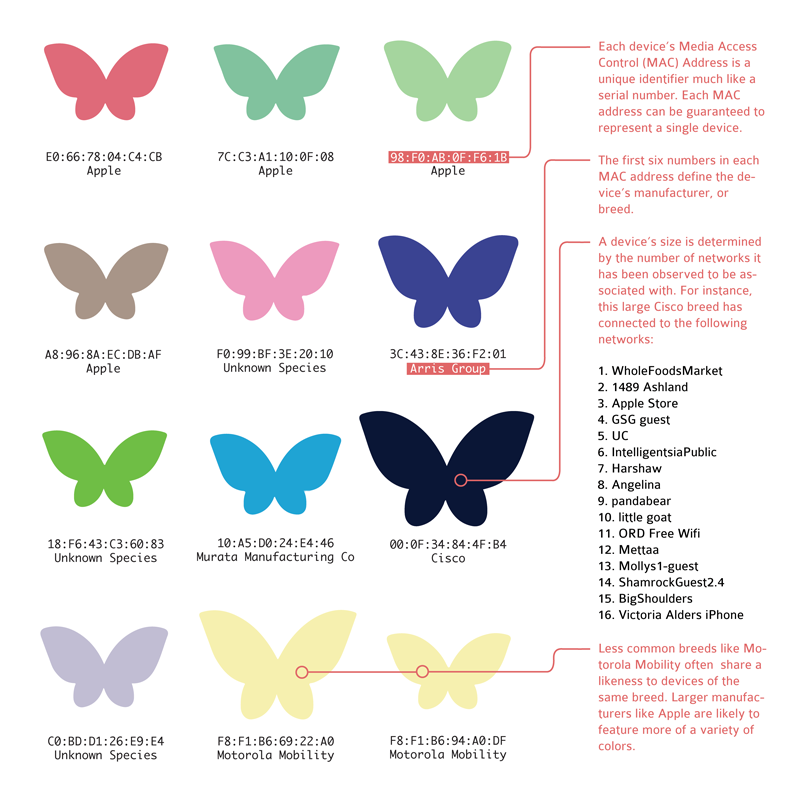
\includegraphics[width=12cm]{images/probekit.png}
	\caption{Démonstration de Probe Kit}
	\label{fig:probekit}
\end{figure}

Avec cette approche ludique, cette démarche vise à sensibiliser les utilisateurs à la recolte passive de données.

\subsection{CrowdProbe}

En plus de la récolte de probe requests, il est possible d'en inférer des données. C'est ce que propose CrowdProbe~\cite{crowdprobe}. 
En installant leur dispositif dans un musée, ils ont réussi à prédire avec une bonne précision le déplacement des utilisateurs, même lors de l'utilisation d'adresse MAC aléatoire.

\begin{figure}[H]
	\centering
	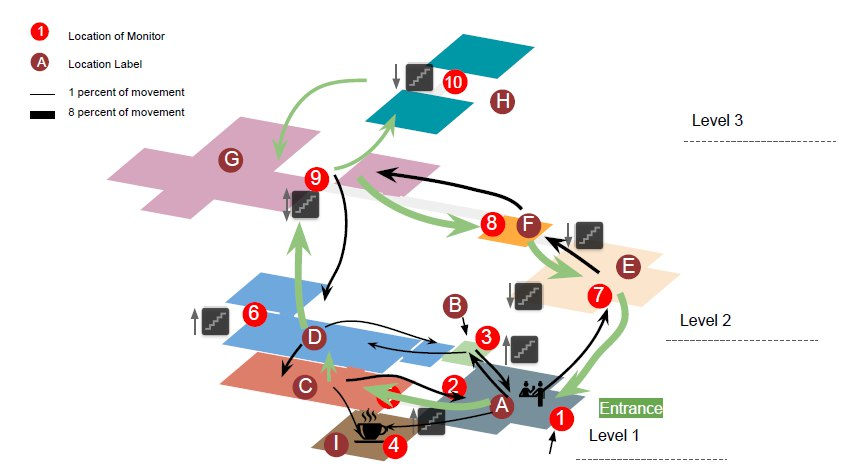
\includegraphics[width=12cm]{images/crowd-probe.jpeg}
	\caption{Flux des visiteurs inféré à l'aide de modèles de Markov}
	\label{fig:crowdprobe}
\end{figure}

\subsection{Serrure déverouillable à l'aide de reconnaissance faciale}
Voici un petit projet~\cite{DOORLOCK} permettant d'utiliser la portabilité de la Raspberry Pi afin de la coupler avec une caméra et une serrure intelligente. 
À l'aide d'OpenCV, le visage de l'utilisateur est reconnu et ouvre la porte si ce dernier est pré-enregistré. 

J'ai inclus ce projet pour montrer qu'il est relativement aisé d'implémenter des mécanismes de reconnaissance faciale à l'aide de la Raspberry Pi


\chapter{Étude sur la législation}
\label{ch:etudelegislation}

Ce travail de Bachelor sera effectué en tant que « proof of concept » et ne sera pas utilisé dans le domaine publique,
mais uniquement dans un environnement contrôlé. C’est pourquoi, il ne sera pas affecté par les différentes
contraintes juridiques exprimées dans cette étude.

Toutefois, à titre informatif et pour démontrer la potentielle nocivité d’un tel système, il a été décidé d’effectuer
une étude sur la légalité et la morale de l’utilisation d’outils de traçage.

Il est à noter que le cadre de cette étude ne comprend que la législation suisse. Les libertés individuelles et le lois sur la protection des données divergent beaucoup
d'un pays à l'autre, c'est pourquoi mes conclusions ne sauraient être valides ailleurs. 

\section{Cas d’utilisation}
Pour circonscrire ce travail dans un cadre juridique, il faut se projeter et prédire les use cases princpaux qu’une
solution telle que WiFace pourrait remplir.

Pour rappel, la solution théorique de Wiface permet d’associer à une identité (Nom, prénom, adresse, informations
personnelles) à un lieu, et à un device.

\subsection{Shopping : Publicité ciblée}

Il serait possible, à l’intérieur d’un grand centre commerciel, de placer plusieurs unités de tracking. Ainsi, le nom et
l’adresse d’un client s’attardant régulièrement devant une enseigne permettrait de la publicité extrêmement ciblée.

Les probe-request donnant également des informations complémentaires directes (constructeur) ou indirectes
(modèle du téléphone), il serait possible pour les vendeurs de matériel informatique de cibler de potentiels nouvaux
acheteurs qui auraient un ancien appareil à remplacer dans un futur proche.

\subsection{Analyse de fréquentation d’un espace publique et prédiction de déplacement}

Lors d’un travail de groupe au MIT, des étudiants ont récoltés plusieurs milions de probe requests et on fait une
analyse de fréquentation de divers lieux clés du campus. Leur projet « Arealytics » les a même conduits à prédire
les prochains déplacements d’un individu en fonction de son trajet courant.
\begin{figure}[H]
	\centering
	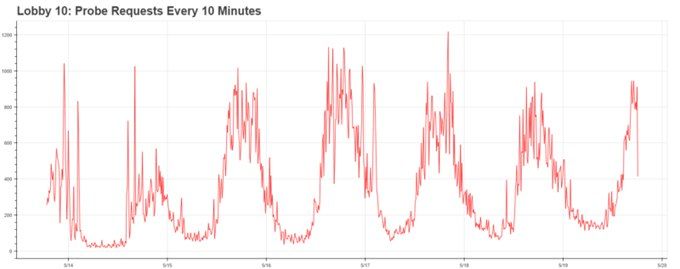
\includegraphics[width=16cm]{images/etude-legi-1.jpg}
	\caption{Arealytics}
	\label{fig:arealytics}
\end{figure}
\begin{figure}[H]
	\centering
	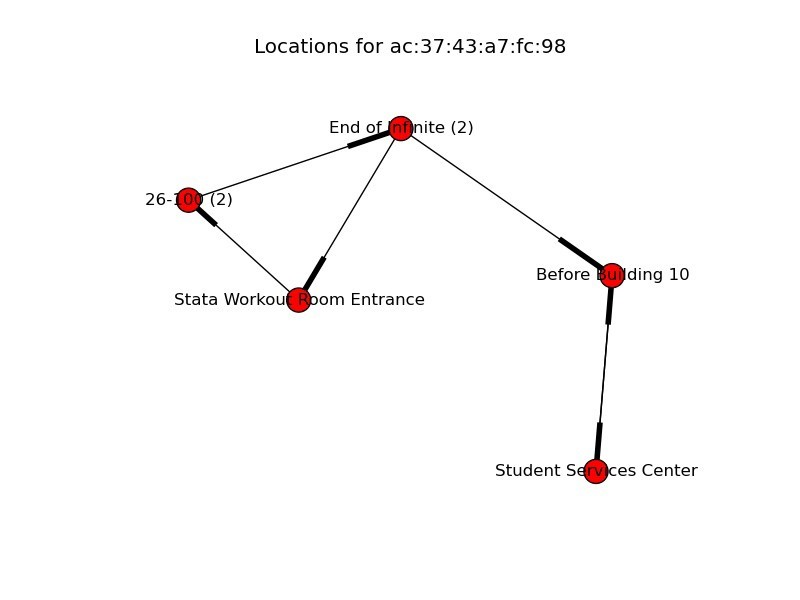
\includegraphics[width=12cm]{images/etude-legi-2.jpg}
	\caption{Arealytics}
	\label{fig:prediction de chemins à l'aide de probe}
\end{figure}

Dans cet exemple, nous voyons que l’utilisation de simple probe request même sans prise d’image donne déjà
énormément d’information brute.

\subsection{Forensique}
La capacité de pouvoir situer un individu, ou un groupe dans un espace géographique donné pourrait être utilisé
comme preuve lors de procès. Par exemple, la présence d’une adresse MAC lors d’un crime, permet avec grande
certitude de s’assurer de la présence de l’appareil associé. Couplé à une caméra, cette technique pourrait
singulièrement améliorer les systèmes de surveillance actuels et proposer de nouveaux outils aux enquêteurs.

\section{Définitions}
Selon la Loi fédérale sur la protection des données (LPD) Section 1, Art 3
On entend par:

\begin{enumerate}[label=\alph*]
\item données personnelles (données), toutes les informations qui se rapportent à une personne identifiée ou
identifiable;
\item personne concernée, la personne physique ou morale au sujet de laquelle des données sont traitées;
\item données sensibles, les données personnelles sur:
\begin{enumerate}[label=\alph*]
\item les opinions ou activités religieuses, philosophiques, politiques ou syndicales,
\item la santé, la sphère intime ou l’appartenance à une race,
\item des mesures d’aide sociale,
\item des poursuites ou sanctions pénales et administratives;
\end{enumerate}
\item profil de la personnalité, un assemblage de données qui permet d’apprécier les caractéristiques essentielles
\item la personnalité d’une personne physique;
\item traitement, toute opération relative à des données personnelles – quels que soient les moyens et procédés
utilisés – notamment la collecte, la conservation, l’exploitation, la modification, la communication,
l’archivage ou la destruction de données;
\item communication, le fait de rendre des données personnelles accessibles, par exemple en autorisant leur
consultation, en les transmettant ou en les diffusant;
\end{enumerate}

Ces quelques définitions vont permettre d’aborder les différentes problématiques dressée par ce travail.

\section{Articles affectant le projet}

Dans cette section, il sera fait mention de plusieurs articles de la LPD permettant de justifier – ou non – la potentielle
mise en place du produit en conditions réelles de par sa licéité.

\subsection{Section 1, Art 3, alinéa 2}
« Leur traitement (des données personnelles) doit être effectué conformément aux principes de la bonne foi et de
la proportionnalité. »

Certains des cas d’utilisations mentionnés ne permettent pas de mettre en œuvre le principe de proportionnalité.
Par exemple, utiliser des mécanismes poussés pour découvrir le moyen de contacter un potentiel client sans
intervention de sa part.

\subsection{Section 1, Art 5, alinéa 1}
«Celui qui traite des données personnelles doit s’assurer qu’elles sont correctes. Il prend toute mesure appropriée
permettant d’effacer ou de rectifier les données inexactes ou incomplètes au regard des finalités pour lesquelles
elles sont collectées ou traitées. »

Au vu des algorithmes qui seraient mis en place, il sera difficile voir impossible de garantir l’exactitude des données
personnelles. Par exemple, l’assignation d’une identité à une adresse MAC à l’aide d’image est un processus
hasardeux qui a de grande chance d’aboutir à une mauvaise labellisation des données personnelles

\subsection{Section 3, Art 12, alinéa 2}
«Personne n’est en droit notamment de:
\begin{enumerate}[label=\alph*]
\item traiter des données personnelles en violation des principes définis aux art. 4, 5, al. 1, et 7, al. 1;
\item traiter des données contre la volonté expresse de la personne concernée sans motifs justificatifs;
\item communiquer à des tiers des données sensibles ou des profils de la personnalité sans motifs justificatifs»
Afin de retrouver l’identité d’une personne, la solution WiFace devra communiquer des informations personnelles
à des tiers (e.g recherche inversée d’image).
\end{enumerate}

\section{Conclusion}
Il est apparent que la plupart des cas d’utilisation ne respectent pas la LPD. Par conséquent, l’implémentation
concrète d’une solution comme WiFace semble compromise sur le marché Suisse.




\chapter{Éthique et moralité des systèmes de surveillance}
\label{ch:etudemoralite}

Au delà de l’aspect législatif abordé dans le chapitre précédent, il est essentiel pour un ingénieur de mesurer ses
responsabilités morales quant aux produits qu’il aide à créer. N’étant pas convenablement formé sur ce sujet, je
me permettrai de me baser sur le travail d’autrui et de faire le lien avec le projet «WiFace».

\section{Positionnement personnel}
À des fins de transparence, j'ai jugé pertinent d'inclure mon positionnement sur la question de la moralité de mon projet,
notamment avant le début de mes recherches.

En tant que technophile, je suis toujours emballé à l'idée de concevoir, développer ou implémenter de nouvelles idées et faire progresser petit à
petit mon savoir. 
Toutefois, dès que le sujet m'a été présenté, je n'ai pu m'empêcher de penser aux conséquences sociétales du développement technologique, 
souvent plus rapide que le développement légistlatif et moral.

Prenons l'exemple évident du système de crédit social en Chine: les outils de surveillance de masse utilisés sont technologiquement très intéressants, mais
beaucoup ressentent un certain malaise quant à leur champs d'application. Dans ce travail de Bachelor, je développe également un outil, sans fixer son cadre d'utilisation.
Je me permets donc d'être vigilant et d'inclure ce chapitre traitant des possibles dérives d'utilisation d'un tel produit. 

\section{La reconnaissance faciale, une technologie déshumanisante}
Dès le début des recherches, il est apparu clairement que la reconnaissance faciale allait être l’aspect soulevant le
plus de questionements moraux dans mon travail, bien plus que l’association d’une identité et d’un terminal.
Pourquoi est-ce le cas ? Les deux situations permettent pourtant de caractériser une personne de manière unique.

Le Prof. Brey, auteur de l'étude "Ethical aspects of facial recognition systems in public places"~\cite{brey_2004}, l’explique en qualifiant le procédé de reconnaissance faciale de «déshumanisant». En effet, pouvoir
encoder le visage (ses features) d’une personne – et donc une partie de son unicité - sur quelques bytes semble
dérangeant pour beaucoup. De plus, un visage est partie intégrante de l’identité d’un individu, alors qu’un terminal
n’est finalement qu’une possession temporaire.

Une autre problèmatique inhérente à cette technologie est celle de l’atteinte à la vie privée et à la confidentialité.
Un système permettant d’identifier, tracer, journaliser et incriminer un individu dans l’espace publique ou privé
nuit gravement aux droits des individus tels que mentionnés dans l’Article 8 de la Convention européenne des droits
de l’homme.

Cette dernière proclame le droit de toute personne au respect « de sa vie privée et familiale, de son domicile et de
sa correspondance », concrétisant ainsi nos questionnements.

\section{L’opposition entre sécurité et confidentialité}
Malgré tout, une part de l’opinion publique approuve l’implémentation de tels systèmes de reconnaissance.
Comme argument principal, nous retrouvons souvent l’augmentation de la sécurité.

L’exemple des passeports bioémtriques est parlant: certains acceptent volontiers son utilisation car les avantages
(lutte contre le terrorisme, usurpation d’identité, augmentation de la facilité de déplacement) semblent
supérieurs aux désavantages (processus déshumanisant, atteinte à la liberté) mais il s’agit d’un cadre très précis, et
ces même personnes ne seraient pas forcément d’accord de trouver de pareils systèmes dans d’autres
circonstances (dans l’espace publique, dans des établissements privés). Cela nous amène donc à la première dérive
: le «Function creep» (dérapage fonctionnel).

\section{Le function creep}
Ce terme, emprunté de l’auteur John Woodward, est le phénomème par lequel une technologie développée dans
un certain but outrepasse ces derniers et élargit son champ d’utilisation. Cela peut être dû à un usage abusif ou
par des changements législatifs la concernant.

L’étude susmentionnée prend l’exemple des Smart CCTV au début des années 2000 (caméras de surveillance
couplées à un système de reconnaissance faciale.) Ces dernières ont été testées par la police afin de retrouver des
personnes disparues et identifier des criminels inscrits dans une base de données.

Cette technologie étant très versatile, il est facile d’imaginer d’autres use-case pour la même implémentation de
ce système. Par exemple, l’utilisation abusive pour le bénéfice personnel d’un agent de police (surveillance de ses
proches, utilisation illégitime des images capturées). Le système initial semblait alors moralement acceptable mais
son dérapage fonctionnel l’a rendu intolérable, pourtant ce dernier n’est pas forcément détectable par les sujets
de cette technologie (le grand public).

\section{La fiabilité et les erreurs}
Comme nous l’avons expliqué, il existe déjà des implémentations servant des systèmes très critiques, pouvant
mener à des arrestations et d’autres conséquences importantes pour ses sujets. Or, bien qu’elle s’améliore avec le temps, la reconnaissance facial est sujette à des erreurs. Dans les systèmes de surveillance, cela amène à une
méfiance générale et à un sentiment d’insécurité. 

Il existe deux types d’erreurs ayant des conséquences différentes:
\begin{enumerate}
\item Le faux négatif : Une personne devant être identifiée ne l’est pas, le système ne remplit pas son objectif et
donc ses désavantages outrepassent ses avantages
\item Le faux positif: Une personne ne devant pas être identifiée est mal reconnue et prise pour quelqu’un
d’autre, le système incrimine une personne innocente / non-concernée, cela décrédibilise le système et
amène à des conséquences néfastes
\end{enumerate}

La deuxième catégorie d’erreur est plus critique que la première, c’est pourquoi la majeure partie des
implémentations choisissent un seuil minimal de confiance très haut même si cela mène à un nombre supérieur de
faux négatifs.

Pour ne rien arranger, il a été montré dans une étude~\cite{Grother2019} effectuée par le NIST (National Institute of Standards and
Technology) que la plupart des meilleures solutions commercialisées de reconnaissance faciale possédent un biais
lié à l’origine du sujet. En effet, le taux d’erreur est 10 à 100 fois supérieurs sur les sujets Afro-Américains et
asiatiques par rapport aux sujets caucasiens.

Un tel biais a le potentiel d’être un facteur d’augmentation de la tension sociale et pourrait impacter la législation
en criminalisant et discriminant injustement certains groupes d’individus par rapport à d’autres.

\section{La vie privée}
Le dérapage fonctionnel et la possibilité d’erreurs n'expriment pas totalement en quoi de telles technologies portent
atteinte à la vie privée.

De manière empirique, nous pouvons remarquer que certaines personnes pensent qu’il est incompatible de lier
espace publique et vie privée, puisque le premier ne pourrait pas exister dans le deuxième, et donc que la
surveillance n’est pas un problème. Pourtant, dans son essai de 1998, l’auteure Helen Nissenbaum argumente le
contraire. Elle affirme que la récolte et le stockage d’informations à l’aide de dispositifs automatisés amènent souvent
à la violation de la vie privée.

Pour appuyer ses propos, elle se base sur deux prémisses:
Premièrement, en sachant que la plupart des gens se sentent surpris ou mécontents quand ils apprennent que leur
données personnelles ont été collectées à leur insu, même dans un espace publique, elle prouve que ces personnes
s’attendaient à un certain respect de leur vie privée, même dans des lieux de vie communs.

Deuxièment, elle affirme que l’automatisation de la récolte des données est bien plus problématique qu’une
surveillance «manuelle» dans l’espace publique et ce à cause de deux pratiques rendues possibles par la
technologie. La première pratique rendue possible est le changement de contexte de l’information une fois
enregistrée (via la vente de données récoltées par exemple). Or l’être humain donne beaucoup d’importance au
contexte quand il délivre une information volontairement (on parle de ses finances à son banquier, de ses
problèmes de santé à son médecin, mais pas inversement). La journalisation des données amène alors à de
potentielles atteintes à la vie privée. La deuxième pratique est « l’aggrégation des données» ou le Big Data.
L’observation individuelle de certaines actions ou habitudes n’a pas vraiment de conséquences, mais lorsque ces
systèmes sont capables de mettre en lien beaucoup d’informations et d’en tirer des corrélations (par exemple à l’aide
du machine learning) de nouvelles informations peuvent être déduites sans le consentement explicite du sujet,
menant à une autre forme d’atteinte.

\section{Conclusion}
Nous avons examiné certaines implications morales d’un système de surveillance et de récolte de données, en
particulier sur la technologie de la reconnaissance faciale. Parmi les problèmes principaux, nous avons identifié:
l’atteinte à la vie privée, le dérapage fonctionnel, et la potentialité d’erreur.

Au moment de sa conception, WiFace ne dispose pas d’un use case établi. Il s’agit d’un outil, sans cadre prédéfini.
Ce constat nous permet d’affirmer qu’il est donc fortement sujet au dérapage fonctionnel, puisque n’importe quelle
personne pourrait facilement déployer cette solution à bas coût pour son bénéfice personnel.

De plus, afin de proposer les fonctionnalités du cahier des charges, WiFace utilise des technologies peu fiables, comme la reconnaissance faciale. 
Il est donc probable que son utilisation amène à des erreurs, ce qui pose un autre
problème éthique.

L’atteinte à la vie privée semble inhérente à tout système de collecte de données automatisées, WiFace ne faisant
pas exception. En permettant de lier un terminal à un utilisateur, nous pouvons facilement imaginer des situations
où cette information pourrait être sortie de son contexte (publicités ciblées, statistiques de fréquentation). Un autre
objectif secondaire de ce travail est la recherche d’informations sur une identité, menant obligatoirement à
l’agglomération de ces données.

D’après ces critères et selon mon appréciation personnelle, je me permets d'affirmer que l’utilisation de ce travail ne respecte pas les standards d’éthique et de déontologie
qu’un établissement comme la HEIG-VD veut s’imposer (conformémant à la charte d'éthique et de déontologie~\cite{HESCHARTE}). Seuls les objectifs pédagogiques et d’évaluation doivent
être visés, et en aucun cas ce travail ne devra mener à la commercialisation d’un futur produit.



\chapter{Étude de marché}
\label{ch:etude-de-marche}

\section{Nano-ordinateurs}

Afin de pouvoir faire fonctionner le prototype développé, il est nécessaire d’utiliser des nano-ordinateurs (un par
caméra), ce qui offre le meilleur compromis entre puissance de calcul, mobilité et prix d’acquisition.

Voici les critères permettant de choisir le modèle à utiliser :
\begin{itemize}
\item Installation libre d’une distribution Linux compatible avec les outils à utiliser (librairies, langages, drivers)
\item Compatibilité hardware avec les cartes réseaux 802.11 et les caméras choisies à la section \ref{sec:choix_camera}
\item Puissance processeur et RAM suffisantes pour exécuter les tâches les plus lourdes du projet (notamment le traitement à l'aide d'OpenCV)
\item Prix adéquat et compatible avec le budget associé au travail de Bachelor
\item Documentation fournie et/ou communauté active
\end{itemize}

Le tableau~\ref{tab:etude-marche-comparatif} résume le comparatif.

\begin{table}[H]
    \resizebox{\textwidth}{!}{%
    \begin{tabular}{@{}p{5cm}p{5cm}p{5cm}p{5cm}@{}}
    \toprule
     & \textbf{NanoPC-T4}\cite{NANOWIKIT4} & \textbf{Raspberry Pi 4}\cite{MANRASP} & \textbf{ODROID-XU4}\cite{MANXU4} \\ \midrule
    \textbf{Installation Libre} & Partielle & Oui & Partielle \\[0.5cm]
    \textbf{Compatibilité caméra} & Module caméra existant & Module caméra existant & Caméra USB \\[0.5cm]
    \textbf{Compatibilité antenne 802.11} & Oui & Oui & Oui \\[1cm]
    \textbf{Spécifications du processeur} & Dual-Core Cortex-A72 (up to 2.0GHz) + Quad-Core Cortex-A53 (up to 1.5GHz) & Broadcom BCM2711, Quad-Core Cortex-A72 (ARM v8) 64-bit SoC @1.5GHz & Samsung Exynos5 Octa ARM Cortex™-A15 Quad 2Ghz and Cortex™-A7 Quad1.3GHz CPUs15 \\
    \textbf{RAM} & Dual-Channel 4GB LPDDR3-1866 & 1GB, 2GB or 4GB LPDDR4-3200 SDRAM & 2GB LPDDR3 RAM at 933MHz \\[1cm]
    \textbf{Prix sans extension} & $\sim$150 \$ & $\sim$65 \$ (Modèle 4GB) & $\sim$80 \$ \\[0.5cm]
    \textbf{Qualité de la documentation} & Un wiki & Communauté très active et beaucoup de documentation & Quelques user guides, un wiki \\ \bottomrule
    \end{tabular}%
    }
    \caption{\label{tab:etude-marche-comparatif}Comparatif des nano-ordinateurs}
    \end{table}

Au vu de la qualité de la documentation, du prix raisonnable du modèle possédant 4GB et de tous les autres critères
remplis, la meilleure alternative pour le projet semble être la \textbf{Raspberry Pi 4}.

\section{Caméra pour la reconnaissance faciale}
\label{sec:choix_camera}

Afin de pouvoir enregistrer des images, pour les traiter et ainsi reconnaître des visages, une caméra devra être
associée à la raspberry pi. Ce use-case étant fréquent, un module caméra officiel\cite{MANRASPCAM} est proposé à la vente. Le tableau~\ref{tab:etude-marche-picamera}
énumère quelques spécifications :

\begin{table}[H]
    \resizebox{\textwidth}{!}{%
    \begin{tabular}{@{}llll@{}}
    \toprule
    \textbf{Prix} & \textbf{Résolution} & \textbf{Modes vidéo} & \textbf{Driver Linux} \\ \midrule
    Environ 25 dollars & 8 Megapixels & \begin{tabular}[c]{@{}l@{}}1080p30, 720p60, \\ 640×480p60/90\end{tabular} & V4L2 driver
    \end{tabular}%
    }
    \caption{\label{tab:etude-marche-picamera}Spécification du module PiCaméra}
\end{table}

Au vu des nombreux projets open-source utilisant ce module pour faire de la reconnaissance faciale, et du fait qu’il
soit un produit agréé, ce dernier sera choisi pour le projet. Il existe également une version V1 de ce module,
proposant des performences moindres, pour un prix sensiblement identique.

\section{Antenne 802.11}

Afin de pouvoir sniffer les probe requests, il faudra une carte WiFi capable de se mettre en mode « Monitor » (pour
recevoir les paquets qui ne sont pas directement adressé à l’adresse de la Raspberry). Comme il sera nécessaire
que la raspberry soit également connectée à internet pour envoyer des données, une antenne supplémentaire sera
utilisée. L’école possède déjà des antennes AWUS036H compatibles, qui permettront d’effectuer le sniffing.





\chapter{Conception}
\label{ch:conception}

\section{La base de données}
\label{sec:database}
Comme des probes requests, des images, et des données personnelles vont être enregistrées et que du traitement
logique leur sera associé, il est important de concevoir une base de donnée claire et bien structurée.

\subsection{Modèle entité-association}
Plusieurs versions du modèle EA ont été imaginées avant d’arriver à la version finale. Afin de mieux cerner les enjeux
de la structure de la base de données, ces dernières vont être commentées. Mais d’abord, listons les différentes
entités

Vendor : Il s’agit du fabricant qui possède un OUI. Étant unique, cet identifiant servira comme clé de la table.

MACAddress : Représente une adresse MAC. Un booléean lui est associé pour savoir si elle semble aléatoire. Une
adresse MAC étant unique (ou presque) elle est utilisée comme clé de la table.

Probe : Représente une probe request. L’heure à laquelle elle a été capturée ainsi que le SSID visé font partie de
l’entité.

Place : Représente l’endroit où la capture a eu lieu.

Picture : Représente une photo prise par le module caméra.

Identity : Représente l’identité d’une personne. On y trouvera les données personnelles récupérées via différents
vecteurs.

BelongsTo: Il s'agit de la relation entre une identité et une MAC adresse. En d'autres mots:
Quelle est la probabilité que la MAC adresse appartienne bien à cette personne ?

Represents: Il s'agit de la relation entre une identité et une image. En d'autres mots:
Quelle est la probabilité que l'image représente bien cette personne ?


\subsubsection{Première version}
Dans cette première ébauche, toutes les entités sont reliées de manière plutôt simpliste. Regardons toutefois
quelques-unes de ces relations.
Une entité « vendor » peut n’avoir délivré aucune adresse MAC puisqu’ils seront tous insérés dans la base de données
à sa création.

Dans ce modèle, visible sur la figure ~\ref{fig:model-ea-1}, une « Identity » est reliée à aucune ou plusieurs MACAddress et photo. (L’individu peut posséder
plusieurs appareils et plusieurs photos ont pu être prises)

\begin{figure}[H]
	\centering
	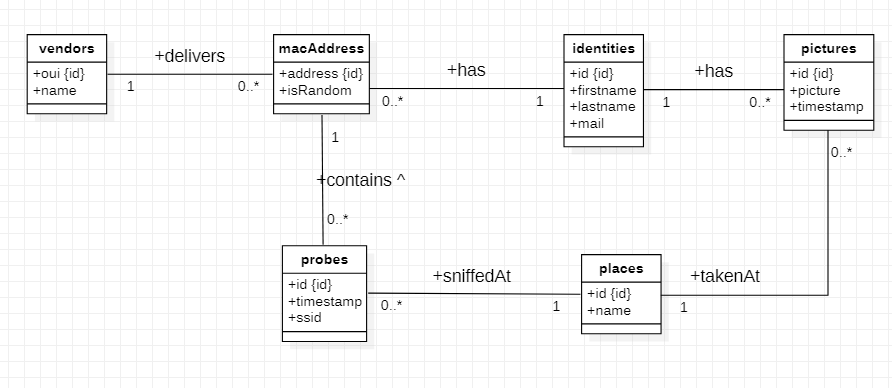
\includegraphics[width=12cm]{images/database_1.png}
	\caption{Première version entité-association}
	\label{fig:model-ea-1}
\end{figure}

Problème : Dans cette conception, il n y a aucune notion de probabilité. Quand une identité a été reliée à une
adresse MAC par exemple, il n’est pas possible de modéliser le doute. Or, dans notre projet, il n y aura que très
peu d'occurences où la certitude est présente. Il faut donc modéliser cette propriété de probabilité.

\subsubsection{Deuxième version – Modélisation des probabilités}
Des relations intermédiaires ont été ajoutées. L’association entre une adresse MAC ou une photo avec une
identité est maintenant « pondérée » par une probabilité. Cette deuxième itération est visible sur la figure ~\ref{fig:model-ea-2}

\begin{figure}[H]
	\centering
	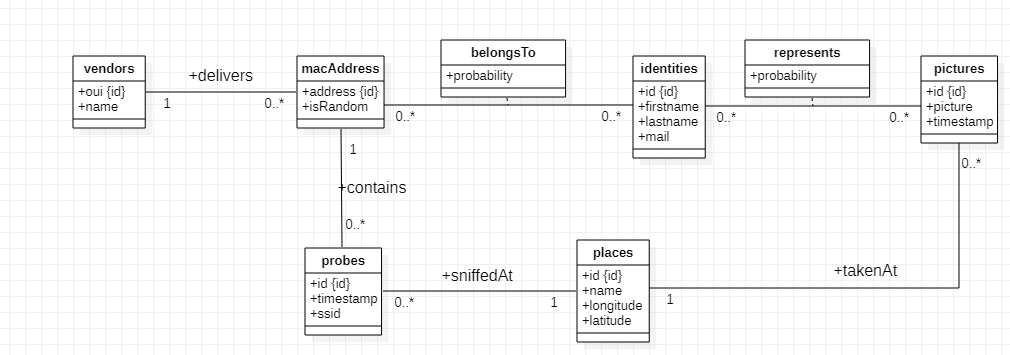
\includegraphics[width=12cm]{images/proto-2.png}
	\caption{Deuxième version entité-association}
	\label{fig:model-ea-2}
\end{figure}

Nouveau problème : Dans ce schéma, il est possible d’obtenir une identité sans image. Or, d’après les
spécifications, ce n’est pas possible puisque c’est grâce à la recherche inversée qu’une identité est établie.

\subsubsection{Troisième version – Identité à partir d’une photographie}

\begin{figure}[H]
	\centering
	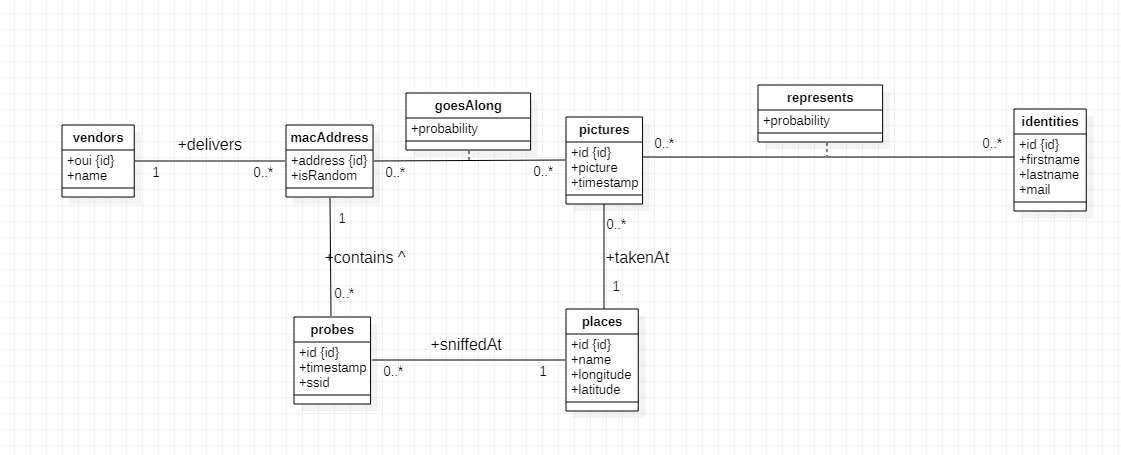
\includegraphics[width=12cm]{images/proto-3.png}
	\caption{Troisième version entité-association}
	\label{fig:model-ea-3}
\end{figure}

Le problème susmentionné a été résolu sur la figure ~\ref{fig:model-ea-3} en détachant l’identité de l’adresse MAC. Seul la photo y est attachée, et
c’est maintenant le lien entre une adresse et une image qui est pondéré.

\subsubsection{Quatrième version – Détails d'une image}

À mi-chemin du projet, il a été remarqué que les données renvoyées par l'API Amazon Rekognition étaient très utiles 
pour implémenter plusieurs fonctionnalités. Ces attributs ont donc été rajoutés à la table Picture.
Ils servent notamment à cibler l'utilisateur (âge, genre, émotions) ou à déterminer la qualité de la photo (sharpness et brightness).
Les nouveaux champs ont été ajoutés sur la figure ~\ref{fig:model-ea-4}

\begin{figure}[H]
	\centering
	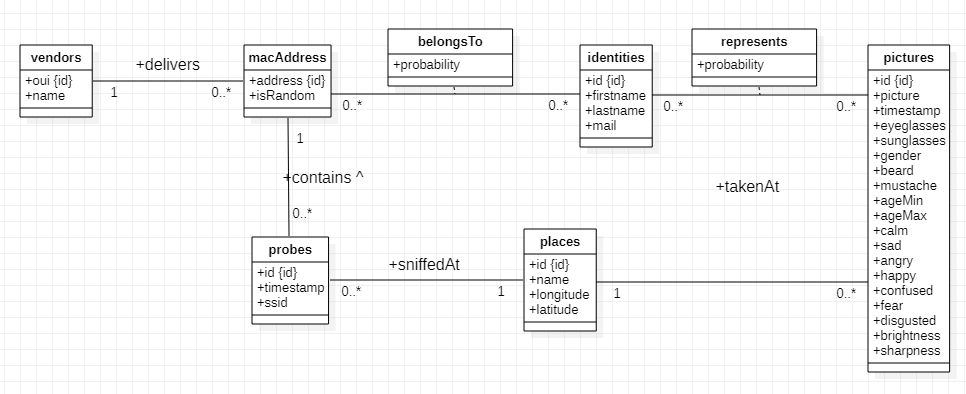
\includegraphics[width=12cm]{images/database_4.png}
	\caption{Quatrième version entité-association}
	\label{fig:model-ea-4}
\end{figure}

\subsubsection{Version finale}

La figure~\ref{fig:model-ea-5} est la version finale du modèle. 
Une entité User a été ajoutée, afin de pouvoir permettre aux clients Raspberry de se localiser.
Un booléean "PP2I" a été ajouté comme attribut de l'entité Identities et MAC Address. Cela permet
d'indiquer si ladite entité doit être incluse dans l'algorithme de mariage PP2I. 

\begin{figure}[H]
	\centering
	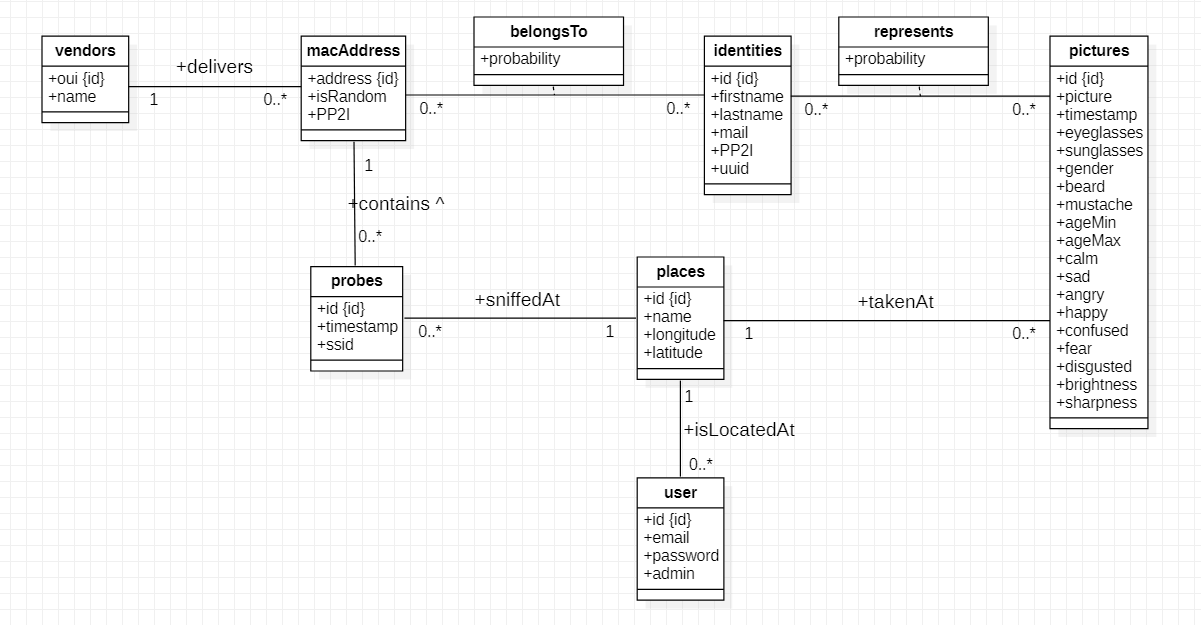
\includegraphics[width=12cm]{images/database_finale.png}
	\caption{Version finale entité-association}
	\label{fig:model-ea-5}
\end{figure}

\section{L'API WiFace}

Afin de développer un projet plus évolutif, sécurisé, et scalable, il a été décidé d'implémenter une API rest permettant les opérations CRUD et d'autres
traitements sur les entités présentées dans la section~\ref{sec:database}.\cite{FLASKREST}
Ainsi, la responsabilité d’effectuer la grande partie de la logique métier pourra
être distribuée au serveur.

Une documentation interactive de toutes les routes est disponible à l'adresse relative \textbf{api/ui} après avoir lancé le serveur~\ref{ch:guide_installation}. 
\section{Le client Raspberry}
Les différents clients Raspberry auront la responsabilité de collecter les informations et de les envoyer
au serveur principal via l'API. 

Pour se faire, elles exécuteront en continu deux processus:
\begin{enumerate}
	\item scanProbe: Récupère les données 802.11 (extraction des MAC Address, du constructeur, analyse de l'aléatoire)
	\item recognizeFace: Analyse des frames de la caméra, si un visage est détecté localement par OpenCV, envoi de l'image à l'API
\end{enumerate}

Ce même client peut être dupliqué autant de fois que nécessaire sans adaptation. 

\section{Dashboard : Visualisation des informations}
Afin qu'un opérateur puisse observer les données récoltées, les données reçues par l'API sont disponibles sous forme de front-end.
Une présentation détaillée des fonctionnalités disponibles est fournie en annexe.

\section{Architecture générale}

L'interaction entre les différents éléments du projet est schématisée sur
la figure~\ref{fig:diag_archi}.

\begin{figure}[H]
	\centering
	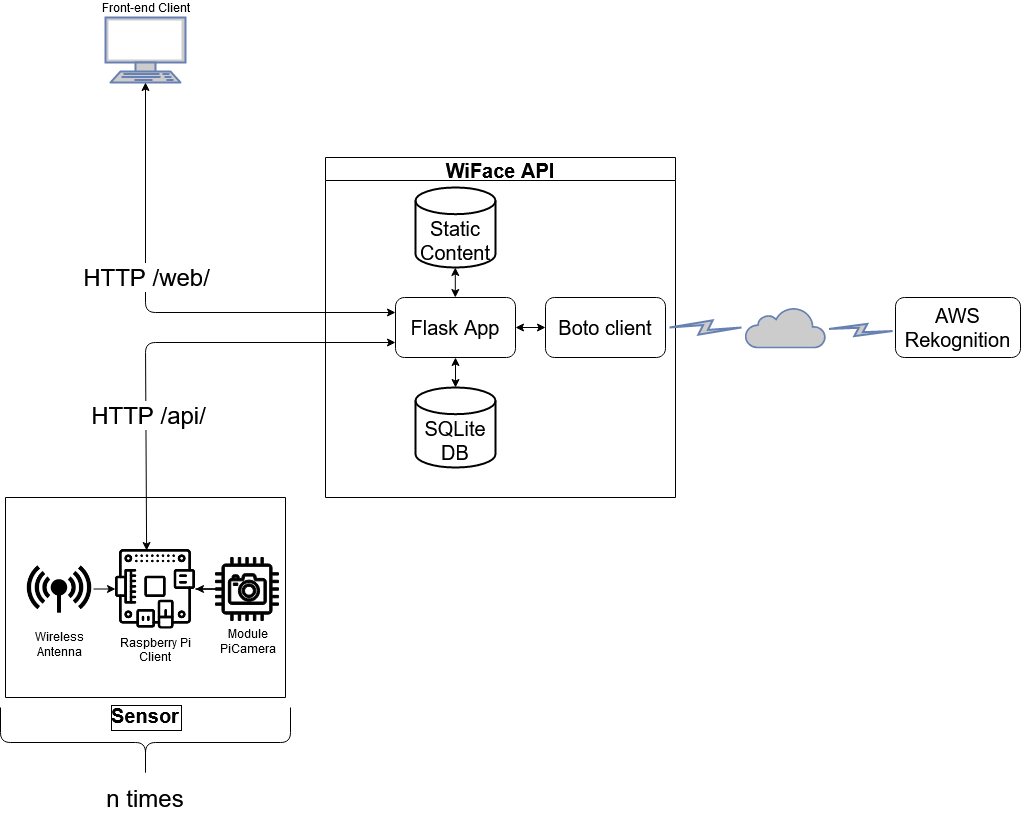
\includegraphics[width=16cm]{images/conception/diagram_archi.png}
	\caption{Diagramme de l'architecture générale}
	\label{fig:diag_archi}
\end{figure}

Les \textbf{sensors} (Client Raspberry Pi, antenne et caméra) s'occupe de récolter les données physiques et de les communiquer à l'API.

Le \textbf{client front-end} peut consulter et gérer les différentes données engrangées par les sensors.

Le point d'entrée de \textbf{l'API WiFace} est \textbf{l'application Flask}. Cette dernière traitera les requêtes
et interagira avec la base de données ou le service Amazon Rekognition si nécessaire.

La \textbf{base de données} permet la persistance des différents éléments (Identités, Utilisateurs, Probe requests récoltées..)

Le \textbf{client "boto"} facilite grandement la communication avec l'API d'Amazon Rekognition, utilisée pour la reconnaissance faciale.


\section{Algorithme PP2I}
L'algorithme PP2I (Probe requests and Pictures to Identity) a la responsabilité d'associer une ou plusieurs adresses MAC à une identité. 
Il a notamment été inspiré d'un travail similaire, sans la composante de reconnaissance faciale.\cite{MACDEAKYN}
Afin d'en analyser le fonctionnement, un lexique doit être établi:
\begin{itemize}
	\item Identité: Personne unique reconnue par l'API Rekognition d'Amazon.
	\item Fenêtre: Intervalle temporel centré autour d'un événement. 
\end{itemize}

Le processus va se dérouler en quatre étapes. 
\begin{enumerate}
	\item Initialisation et incrémentation
	\item Décrémentation majeure dûe à l'absence de l'adresse MAC
	\item Décrémentation mineure dûe à l'absence de la photo
	\item Normalisation des scores
\end{enumerate}

\subsection{Initialisation}
Dans cette phase de l'algorithme, toutes les identités incluses dans l'algorithme (ayant l'attribut PP2I valant True) sont parcourues.
Pour chaque identité, toutes les photos correspondantes sont mises en relation avec probes requests dont l'adresse MAC est inclue dans l'agorithme.
Si un couple (photo, probe request) se trouve dans la même fenêtre, alors on initialise le couple et on l'ajoute au dictionnaire.

\begin{algorithm2e}[H]
	\SetAlgoLined
	\KwIn{List of pictures timestamped and labeled with corresponding identity, list of probe request timestamped}
	\KwResult{Dictionnary containing (adress, identity) tuple as key and probability as value}
	$dict\_couple  \gets \emptyset $\;
	\ForEach(){Identity \textbf{in} AllIdentities}{
		\If(){\textbf{not} Identity.PP2I}{
			$continue$
		}
		 \ForEach(){Picture \textbf{in} Identity}{
			 $beginning \gets Picture.timestamp - half\_window\_duration$\;
			 $end \gets Picture.timestamp + half\_window\_duration$\;
			 $place \gets Picture.place$\;
			 \ForEach(){Probe \textbf{taken at} $place$ \textbf{between} beginning \textbf{and} end \textbf{in} allProbes}{
				\If(){Probe.mac.PP2I}{
			 		$dict\_couple.add(key=(address, identity), value=init\_score)$
			 	}
			}
		}
	}
	\Return{$dict\_couple$}
	\caption{Initialisation et création de couples}
\end{algorithm2e}

\subsection{Décrémentation majeure dûe à l'absence de l'adresse MAC}
Dans cette phase, nous regardons pour un couple donné, si il y a des instances où l'on trouve 
l'identité (une photo) sans l'adresse MAC (une probe request). Comme c'est un cas peu probable si le couple
est correct (une probe request est plus facilement récupérable qu'une photo), on descend beaucoup le score du couple si cela arrive.

\begin{algorithm2e}[H]
	\SetAlgoLined
	\KwIn{$dict\_couple$, list of pictures timestamped and labeled with corresponding identity, list of probe request timestamped}
	\KwResult{Dictionnary containing (adress, identity) tuple as key and probability as value}
	$mac\_addresses  \gets \emptyset $\;
	\ForEach(){Couple \textbf{in} $dict\_couple$}{
		 \ForEach(){Picture \textbf{representing} Couple[Identity]}{
			$beginning \gets Picture.timestamp - half\_window\_duration$\;
			$end \gets Picture.timestamp + half\_window\_duration$\;
			$place \gets Picture.place$\; 
			\ForEach(){Probe \textbf{taken at} $place$ \textbf{between} beginning \textbf{and} end \textbf{in} allProbes}{
				$mac\_addresses.add(Probe.mac)$
			 }
			}
		\If(){Couple[mac] \textbf{not in} $mac\_addresses$}{
			$dict\_couple[(adress, identity)]$ -= $BigMalus$\;
		}

		}
	\Return{$dict\_couple$}
	\caption{Décrémentation majeure dûe à l'absence de l'adresse MAC}
\end{algorithm2e}


\subsection{Décrémentation mineure dûe à l'absence de la photo.}
Dans cette phase, nous regardons pour un couple donné, si il y a des instances où l'on trouve 
l'adresse MAC (une probe request) sans l'identité (une photo). Comme c'est un cas fréquent, on ne baissera qu'un peu le couple donné. 


\begin{algorithm2e}[H]
	\SetAlgoLined
	\KwIn{$dict\_couple$, list of pictures timestamped and labeled with corresponding identity, list of probe request timestamped}
	\KwResult{Dictionnary containing (adress, identity) tuple as key and probability as value}
	$identities  \gets \emptyset $\;
	\ForEach(){Couple \textbf{in} $dict\_couple$}{
		 \ForEach(){Probe \textbf{containing} Couple[address]}{
			$beginning \gets Probe.timestamp - half\_window\_duration$\;
			$end \gets Probe.timestamp + half\_window\_duration$\;
			$place \gets Probe.place$\; 
			\ForEach(){Picture \textbf{taken at} $place$ \textbf{between} beginning \textbf{and} end \textbf{in} allPictures}{
				$identities.add(Picture.identity)$
			 }
			}
		\If(){Couple[identity] \textbf{not in} $identities$}{
			$dict\_couple[(adress, identity)]$ -= $BSmallMalus$\;
		}

		}
	\Return{$dict\_couple$}
	\caption{Décrémentation mineure dûe à l'absence de la photo}
\end{algorithm2e}

\subsection{Normalisation}~\cite{SKLEARNMINMAX}
Afin de faciliter le traitement, les scores seront normalisés dans un interval [0;1].
Pour ce faire, toutes les adresses candidates à une identités sont sélectionnées et mises à l'échelle entre elles à l'aide de la formule suivante:

\begin{listingsbox}{python}{Formule de normalisation}
X_std = (X - X.min) / (X.max - X.min)
X_scaled = X_std * (max_range - min_range) + min_range
\end{listingsbox}

\chapter{Reconnaissance faciale}
\label{ch:reco_faciale}

Une partie critique du projet consiste à pouvoir identifier des personnes en fonction des images capturées par la
caméra. La reconnaissance faciale étant un sujet d’étude très complexe, il sera nécessaire d’utiliser des solutions
clés en main afin de pouvoir l’incorporer dans l’ensemble du projet. Il peut toutefois être intéressant de
comprendre les bases et les implications de cette technologie.

\section{Une petite touche de théorie}
La reconnaissance faciale utilise la technologie du Machine Learning, et plus précisement du Deep Learning.
Le principe consiste à l’extraction de données intéressantes d’une image (les caractérstiques) afin de créer ou lier une
« empreinte biométrique » à un visage. Ce processus est exemplifié dans la figure ~\ref{fig:reco-process} . Par exemple en mesurant l’écartement des yeux, la longeur du nez, la
profondeur des orbites, on obtient des données uniques qui permettront d’identifier la même personne sur une
image différente.

Les cas d’utilisation de la reconnaissance faciale sont nombreux.
En voici une liste non-exhaustive :
\begin{itemize}
\item identification l’utilisateur d’un téléphone (Apple FaceID),
\item aide à la recherche des personnes disparues,
\item aide aux personnes malvoyantes (détection et notification du sourire de ses interlocteurs),
\item labellisation des personnes sur les réseaux sociaux,
\item lutte contre le terrorisme.
\end{itemize}

\begin{figure}[H]
	\centering
	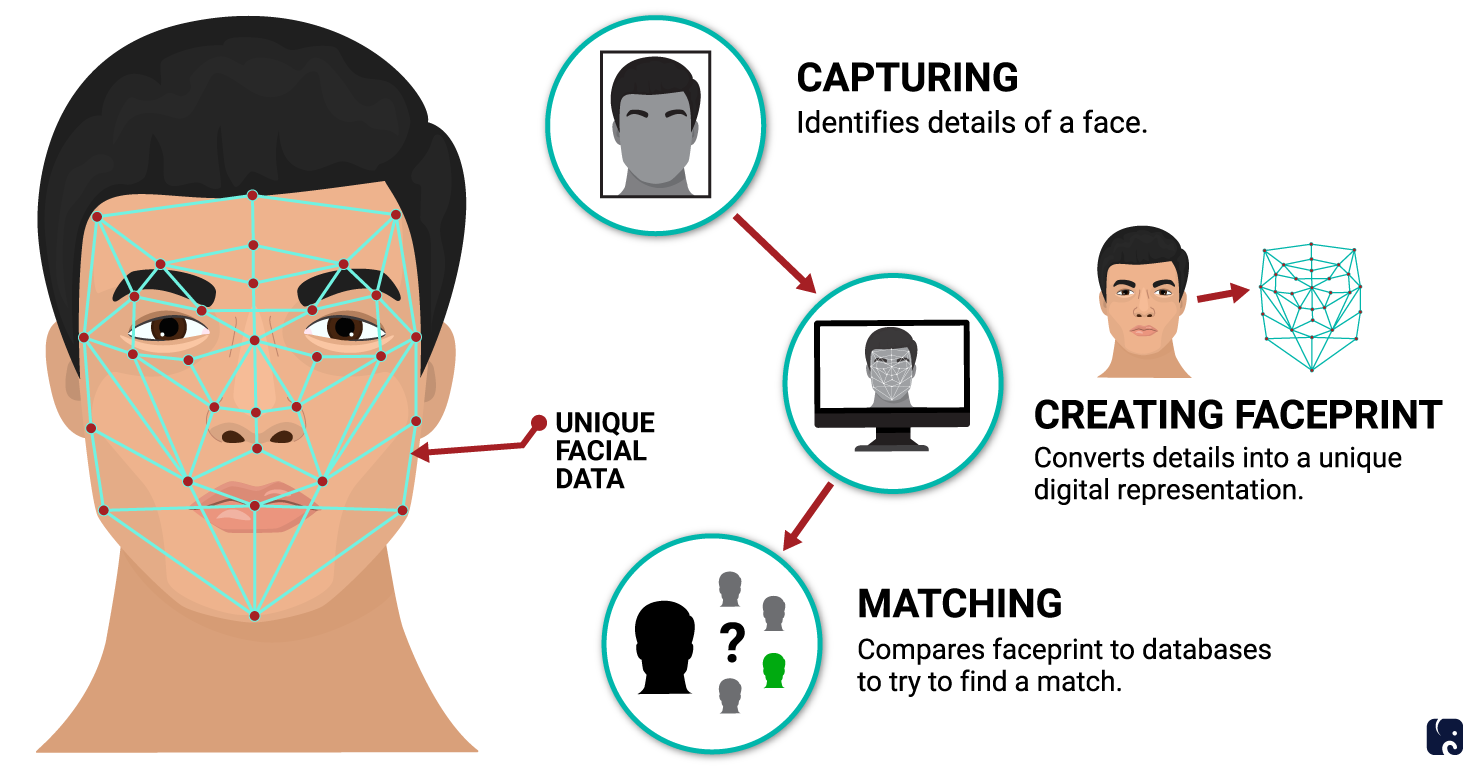
\includegraphics[width=12cm]{images/proto-5.png}
	\caption{Processus de reconnaissance faciale}
	\label{fig:reco-process}
\end{figure}

\section{Choix de la solution}

À l'aide de quelques valeurs clés (précision, rappel, nombre de faux-positifs, ...) nous allons comparer plusieurs solutions existantes et "clés en main" de reconnaissance faciale.
La figure ~\ref{fig:tab-comparatif-reco} ci-dessous énumère les fonctionnalités offertes par les diverses solutions du marché.

\begin{figure}[H]
	\centering
	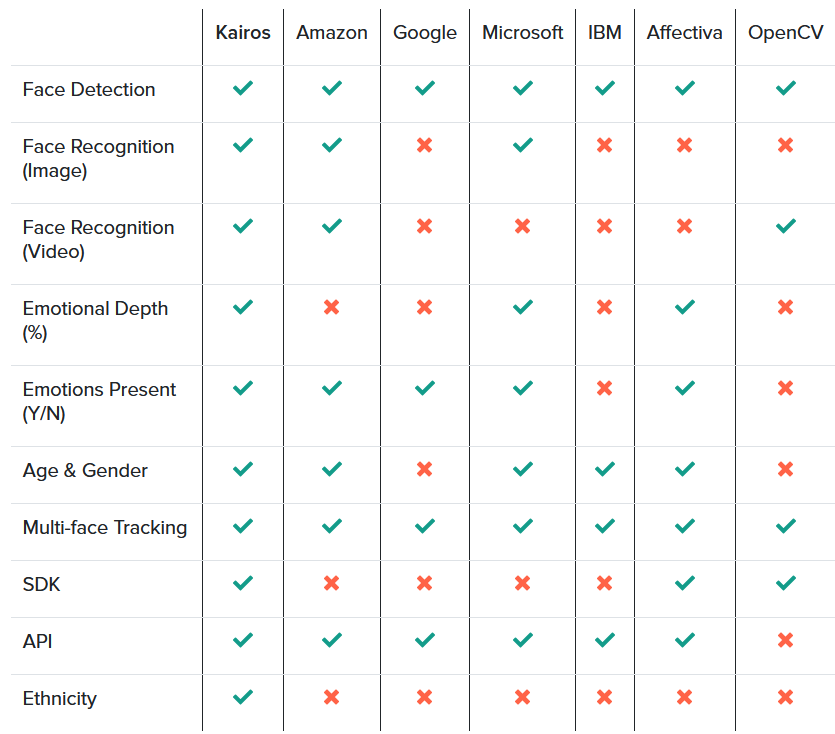
\includegraphics[width=12cm]{images/proto-4.png}
	\caption{Tableau comparatif de solution de reconnaissance faciale}
	\label{fig:tab-comparatif-reco}
\end{figure}

Ce qui est nécessaire, c’est la « Face recognition » sur image (plus compatible avec la notion d’IoT qu’un flux vidéo
complet.) Les trois solutions le proposant sont :

\begin{itemize}
\item Kairos
\item Amazon AWS : Rekognition
\item Microsoft Azure : Face
\end{itemize}

Trois facteurs sont alors importants dans le cadre du projet : La précision, le prix et la facilité d’utilisation.

\subsection{Performances}
Concernant la précision, on peut la mesurer à l’aide des concepts de True Positive (Un visage est correctement
identifié), True Negative (Un visage est correctement exclu), False Positive (Un visage est identifié en tant qu’un
autre) et False Negative (Un visage n’a pas été identifié comme connu)

Une source a utilisé un dataset de visage de l’université de Essex afin de mesurer ces valeurs dans différents
contextes pour les trois solutions. Voici les résultats principaux.

\begin{itemize}
\item Precision (TP/(TP+FP)
\item Recall (TP/(TP+FN))
\end{itemize}

\begin{table}[H]
	\resizebox{\textwidth}{!}{%
	\begin{tabular}{@{}lllllll@{}}
	\toprule
	\textbf{Provider} & \textbf{TP} & \textbf{FP} & \textbf{TN} & \textbf{FN} & \textbf{Precision} & \textbf{Recall} \\ \midrule
	Kairos & 108 & 0 & 150 & 42 & 100\% & 72\% \\
	Microsoft cognitive services & 131 & 0 & 150 & 19 & 100\% & 87.3\% \\
	AWS rekognition & 149 & 0 & 150 & 1 & 100\% & 99.3\% \\ \bottomrule
	\end{tabular}%
	}
	\caption{Seuil de confiance AWS rekognition: 95\% Microsoft: 80\% Kairos: 95\%}
	\end{table}

\begin{table}[H]
	\resizebox{\textwidth}{!}{%
	\begin{tabular}{@{}lllllll@{}}
	\toprule
	\textbf{Provider} & \textbf{TP} & \textbf{FP} & \textbf{TN} & \textbf{FN} & \textbf{Precision} & \textbf{Recall} \\ \midrule
	Kairos & 148 & 0 & 150 & 2 & 100\% & 98.7\% \\
	Microsoft cognitive services & 137 & 0 & 150 & 13 & 100\% & 91.3\% \\
	AWS rekognition & 150 & 2 & 148 & 0 & 98.7\% & 100\% \\ \bottomrule
	\end{tabular}%
	}
	\caption{Seuil de confiance AWS rekognition 70\% Microsoft: 50\% Kairos: 70\%}
	\end{table}

\begin{table}[H]
	\resizebox{\textwidth}{!}{%
	\begin{tabular}{@{}lllllll@{}}
	\toprule
	\textbf{Provider} & \textbf{TP} & \textbf{FP} & \textbf{TN} & \textbf{FN} & \textbf{Precision} & \textbf{Recall} \\ \midrule
	Kairos & 150 & 19 & 131 & 0 & 88.7\% & 100\% \\
	Microsoft cognitive services & 137 & 10 & 140 & 13 & 93.2\% & 91.3\% \\
	AWS rekognition & 150 & 2 & 148 & 0 & 98.7\% & 100\% \\ \bottomrule
	\end{tabular}%
	}
	\caption{Seuil de confiance AWS rekognition: 50\% Microsoft: 30\% Kairos: 50\%}
	\end{table}
Parmi ces résultats, nous pouvons voir que rekognition se démarque par son absence presque totale de FN et un
taux faible de faux positifs, même avec un seuil de confiance bas (ce qui est un avantage dans un environnement
moyennement précis tel que la raspberry).

\subsection{Tarification}

Concernant la tarfication, Amazon et Microsoft se démarquent de Kairos grâce à leur prix moins élevés, et à des
solutions gratuites.

\subsubsection{Kairos}

Kairos pratique des prix mensuels fixes ainsi qu’un supplément par transaction. Par exemple, l’offre « Student
Cloud » coûte 19\$ par mois + 0.02\$ par transaction, avec toutefois 2 semaines d’essai gratuites.

\subsubsection{Microsoft Azure Face}\cite{PRICEAZURE}

Microsoft propose deux solutions : « Free - Web/Container » et « Standard - Web/Container ». Il est à noter que l'échelon gratuit ne comprend pas le « Face Storage » et que l’entraînement est compté dans les transactions (1
transaction / 1000 images utilisées pendant l’entrainement)


\begin{table}[H]
	\resizebox{\textwidth}{!}{%
	\begin{tabular}{@{}llll@{}}
	\toprule
	Instance & Transactions Per Second (TPS) & Features & Price \\ \midrule
	Free & 20 TPM & \begin{tabular}[c]{@{}l@{}}Face Detection\\ Face Verification\\ Face Identification\\ Face Grouping\\ Similar Face Search\end{tabular} & 30K transactions fer per month \\[2cm]
	\multirow{2}{*}{Standard} & \multirow{2}{*}{10 TPS} & \begin{tabular}[c]{@{}l@{}}Face Detection\\ Face Verification\\ Face Identification\\ Face Grouping\\ Similar Face Search\end{tabular} & \begin{tabular}[c]{@{}l@{}}0-1M transactions : 1 USD per 1,000 transactions\\ 1M-5M transactions : 0.80 USD per 1,000 transactions\\ 5M-100M transactions : 0.60 USD per 1,000 transactions\\ 100M+ transactions : 0.40 USD per 1,000 transactions\end{tabular} \\
	 &  & Face Storage & 0.01 USD per 1,000 faces per month \\ \bottomrule
	\end{tabular}%
	}
	\end{table}

\subsubsection{Amazon AWS rekognition}
Rekognizion est compris dans l’offre gratuite d’AWS durant les 12 premiers mois d’utilisation et ce pour 5'000
transactions ainsi que 1'000 métadonnées par mois.

\begin{table}[H]
	\resizebox{\textwidth}{!}{%
	\begin{tabular}{@{}lll@{}}
	\toprule
	\textbf{Type de coût} & \textbf{Tarification} & \textbf{Prix pour 1000 images} \\ \midrule
	Premier million d’images traitées par mois & 0,001 \$ / image & 1 USD \\
	9 millions d’images traitées suivants par mois & 0,0008 \$ / image & 0,8 USD \\
	90 millions d’images traitées suivants par mois & 0,0006 \$ / image & 0,6 USD \\
	Plus de 100 millions d’images traitées par mois & 0,0004 \$ / image & 0,4 USD \\ \bottomrule
	\end{tabular}%
	}
	\caption{Tarification d'Amazon Rekognition}
\end{table}

\subsection{Facilité d’utilisation}
Concernant la facilité d’utilisation, une documentation de bonne qualité semble disponible pour Microsoft et
Amazon. Toutefois, il semble très important pour Microsoft d’avoir des photos d’entraînements avant le processus
de reconnaissance, ce qui ne répond pas au cahier des charges.

\subsection{Choix de la solution}
Grâce aux différents facteurs analysés, c’est la solution d’Amazon (Rekognition) qui a été retenue pour ce projet. À
l’aide d’un échelon gratuit (majoritairement suffisant pour la période de développement), de très bonnes performances
et d’un use case compatible avec le cahier des charges, nous pouvons affirmer qu’il est pertinent de faire ce choix.

\section{Amazon Rekognition : présentation}
Comme expliqué précédemment, Amazon rekognition est un service de reconnaissance d’images. Bien que nous
utilisons seulement les fonctionnalités concernant les visages, il est aussi possible par exemple d’identifier du texte,
des objets ou encore des images inappropriées (contenu explicite et suggestif).

\subsection{Concepts et opérations}
Pour pouvoir utiliser Rekognition, il faut connaître les opérations principales de l’API et en comprendre les concepts
principaux.

\underline{Features} (caractéristiques) : En machine learning, les caractéristiques sont les variables d’entrées permettant de
simplifier le problème et sur lesquelles nous allons nous baser pour faire des classifications. Par exemple, pour la
détection de visages, certaines des caractéristiques sont : écartement des yeux, couleur des yeux, la longueur du
nez, la forme des joues, la profondeur des orbites, ou encore la largeur de la mâchoire. La combinaison de ces
caractéristiques permettent souvent d’identifier de manière unique un individu.

\underline{Collection} : Les collections sont des « conteneurs » AWS server-side qui rassemblent les informations (métadata)
des visages ajoutés. Une collection est identifiée par un ARN (Amazon Resource Name) unique et peut être créée
grâce à l’opération « CreateCollection »

\underline{IndexFace} : Opération d’ajout d’un ou plusieurs visages (métadatas) dans une collection. En entrée, il faut
principalement une image (blob), le nom de la collection dans laquelle insérer les visages, le nombre maximum de
visages à indexer (les visages sont indexés du plus petit au plus grand. Ainsi, sur une image contenant 5 personnes,
si le paramètre vaut 2, seulement les 2 plus grands visages seront ajoutés à la collection)

\underline{SearchFacesByImage}\label{text:SearchFacesByImage} : Opération prenant une image en entrée, récupère le visage le plus visible et cherche dans
une collection donnée si ce visage est reconnu. Si c’est le cas, on peut alors inférer que l’image représente la même
personne que les métadonnées correspondantes.

La figure~\ref{fig:reko-workflow} présente un workflow détaillé d’Amazon Rekognition

\begin{figure}[H]
	\centering
	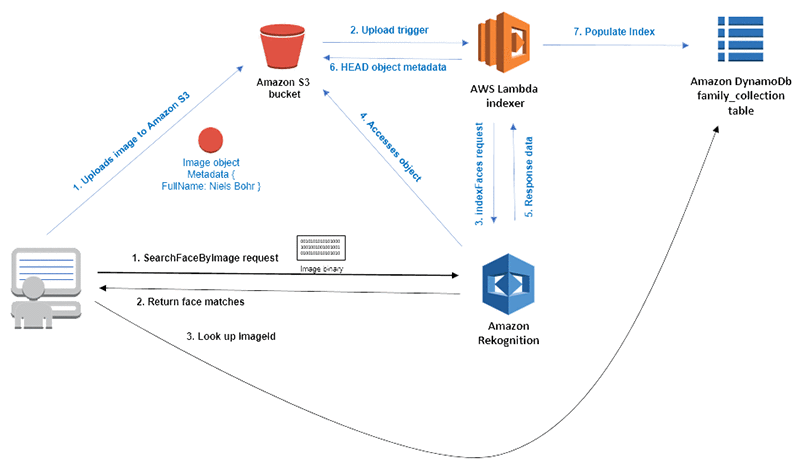
\includegraphics[width=12cm]{images/proto-6.png}
	\caption{Workflow d'Amazon Rekognition}
	\label{fig:reko-workflow}
\end{figure}

\subsection{Prérequis}

Afin de pouvoir travailler avec Amazon Rekognizion, il est nécessaire d’avoir une clé d’authentification à leur API.
Pour cela, il faut créer un compte et s’inscrire au service. Pour cela, merci de suivre la section "Getting started" de la documentation
officielle AWS rekognition~\cite{AWSDOCS}. Une fois la clé obtenue, nous allons utiliser leur SDK pour
Python : boto3. Il suffit alors de mettre ses identifiants dans le fichier config.py du projet. (cf~\ref{ch:guide_installation}) 

\chapter{Adresses MAC et probes requests}
\label{ch:probe_req}

Afin de pouvoir détecter et tracer les différents périphériques réseau présents
pendant les scans, il est impératif de pouvoir les identifier de manière unique et irrévocable.

Pour cela, nous allons utiliser l'adresse MAC. 
Cet identifiant unique peut être récupéré de plusieurs manières, mais ce sont les \textbf{probe requests}
qui vont nous offrir la plus grande souplesse. 

Explorons ces deux concepts.

\section{Adresse MAC, un identifiant pas si unique}

\subsection{Définition:}~\cite{wiki:mac}

"Une adresse MAC (Media Access Control1), parfois nommée adresse physique, est un identifiant physique 
stocké dans une carte réseau ou une interface réseau similaire. À moins qu'elle n'ait été modifiée par l'utilisateur, elle est unique au monde. 

MAC constitue la partie inférieure de la couche de liaison (couche 2 du modèle OSI). Elle insère et traite ces adresses au sein des trames transmises. Elle est parfois appelée adresse ethernet, 
UAA (Universally Administered Address), BIA (Burned-In Address), MAC-48 ou EUI-48."

\subsection{Format}

Les 48 bits d'une adresse sont schématisés sur la figure ~\ref{fig:macstruct} et formatés comme suit :

\begin{figure}[H]
	\centering
	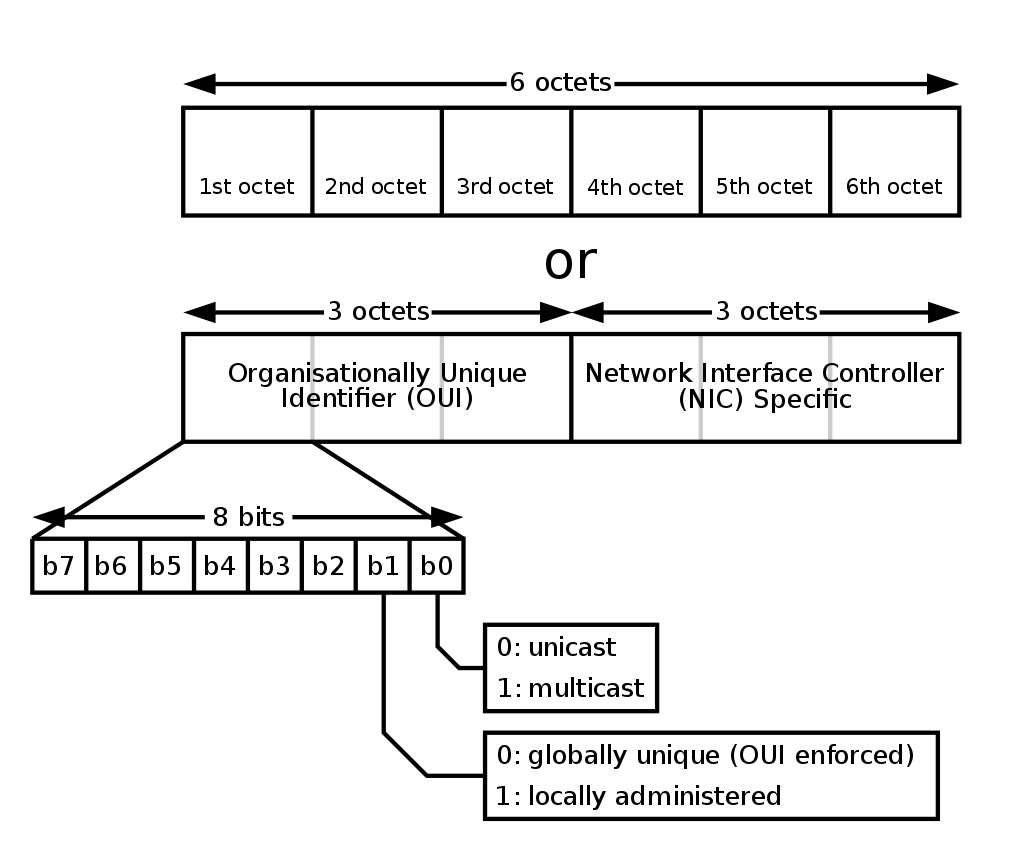
\includegraphics[width=12cm]{images/probe/mac_struc.png}
	\caption{Structure de l'adresse MAC}
	\label{fig:macstruct}
\end{figure}

Les 3 octets de poids faible sont variables et change pour chaque carte mère, c'est ce qui rend chaque adresse du même
constructeur unique, il s'agit du \textbf{NIC}.

Les 3 octets de poids fort sont presque fixes pour chaque constructeur, il s'agit du \textbf{OUI}.
Toutefois, les deux bits de poids faible du premier octet peuvent varier (b1 et b0 sur l'illustration).

b0 indique si l'adresse est individuelle, auquel cas le bit sera à 0 (pour une machine unique, unicast) 
ou de groupe (multicast ou broadcast), en passant le bit à 1.

b1 indique 0 si l'adresse est universelle (conforme au format de l'IEEE) ou 
locale, 1 pour une adresse administrée localement (ce bit sera crucial concernant l'analyse de la randomisation)

\subsection{Problèmes de vie privée et randomisation}
La propriété d'unicité des adresses MAC soulève évidemment des problématiques liées à la vie privée. 
Par exemple, selon les dires d'Edward Snowden, la NSA se servait des adresses MAC afin de
monitorer les déplacements d'individus.~\cite{hackernews:snowdan}

Le sujet de ce travail de bachelor soulève les même problématiques. Par conséquent, certaines marques
ont mis en place la \textbf{MAC Address randomization}.

\subsection{Randomisation des adresses MAC}~\cite{connected:macrandom}

Depuis 2014, de plus en plus de constructeurs ont adoptés des mesures
afin de protéger la véritable adresse MAC de l'appareil. 

\begin{itemize}
    \item iOS à partir d’iOS 8 ;
    \item Windows depuis Windows 10 ;
    \item Android depuis Android 6.0 (un patch gère également Android 5.0 pour certains appareils) ;
    \item certains drivers Linux depuis le kernel 3.18.
\end{itemize}

L'objectif étant de varier suffisamment régulièrement l'adresse pour empêcher le traçage. 
Le processus de randomisation n'étant pas strictement standardisé, l'implémentation peut varier pour chaque constructeur. 

Certaines de ces implémentations sont bonnes (iOS randomise les 6 octets de l'adresse MAC, sauf b1 et b0) alors que d'autres le sont moins (Android possède des OUI fixes pendant la randomisation, ce qui 
permet déjà la divulgation d'informations sur l'appareil.)

\subsubsection{Problèmes liés à l'implémentation de la randomisation}

Bien que le concept de randomisation soit une bonne avancée dans le domaine de la privacy, quelques
problèmes d'implémentation ont mitigé cette dernière. 

Parmi les problèmes récurrents, il a été trouvé:
\begin{itemize}
	\item Mauvais PRNG (le biais permet de faire des liens logiques entre les adresses)
	\item Numéros de séquence augmentant de manière monotone, permettant de faire le lien entre deux adresses aléatoires (cf~\ref{fig:seqnumber})
	\item Les adresses réelles sont parfois divulguées (e.g si l'écran est allumé)
	\item Les timings de scans des appareils peuvent permettre un rapprochement entre plusieurs adresses
	\item Fingerprinting possible à l'aide des Informations Elements (IE)
	\item Beaucoup de méthodes de randomisation ne sont utilisées que lors du scan. Lorsque l'appareil est connecté, ce dernier utilise à nouveau
	sa vraie adresse physique.
\end{itemize} 

Tous ces points s'améliorent avec le temps. 
Par exemple, la nouvelle version d'iOS (14) datant de l'été 2020 permet la randomisation même lorsque l'appareil est connecté.
Cette feature est d'ailleurs mise en avant par Apple, au travers des notifications. \cite{APPLESUPPPRIVATE} 

\begin{figure}[H]
	\centering
	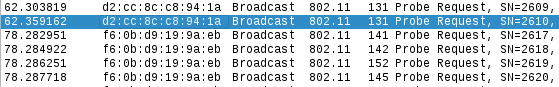
\includegraphics[width=12cm]{images/probe/sn.png}
	\caption{Le changement d'adresse MAC aux lignes 2 et 3 peut être déduit à cause du séquence number proche.}
	\source{~\cite{connected:macrandom}}
	\label{fig:seqnumber}
\end{figure}

\subsection{Détection passive de la randomisation}

\subsubsection{Le bit Locally Assigned}
Le travail WiFace utilise plusieurs méthodes pour détecter la randomisation des adresses MAC. 
La première consiste simplement à contrôler le bit \textbf{b1}, si ce dernier est à 1, cela implique qu'il
y a de grandes chances que l'adresse soit aléatoire. Cependant, ce n'est pas totalement vrai, c'est pourquoi
d'autres techniques sont employées en concert avec celle-ci. 

Dans un corpus datant de fin 2015, l'étude ~\cite{ASMARMD} a demontré les statistiques visibles dans le tableau~\ref{tab:locally_stats}: 

\begin{table}[H]
	\resizebox{\textwidth}{!}{%
	\begin{tabular}{@{}lll@{}}
	\toprule
	\textbf{Category} & \textbf{Subcategory} & \textbf{Number of MACs} \\ \midrule
	\multirow{5}{*}{Locally Assigned} & Total & 1400753 \\
	 & Randomized & 1388656 \\
	 & Service & 4371 \\
	 & Malformed & 6895 \\
	 & Unknown & 831 \\ \bottomrule
	\end{tabular}%
	}
	\caption{Statistiques sur la randomisation - Locally Assigned bit}
	\label{tab:locally_stats}
	\end{table}

Près de 99\% des adresses assignées localement étaient également aléatoires. La consultation
du bit b1 est donc une bonne estimation heuristique. Il est tout de fois intéressant de pouvoir afiner
la détection afin d'obtenir d'autres informations sur le périphérique. 

\subsubsection{Le préfixe DA:A1:19}
Ce préfixe peut être retrouvé lors de la randomisation des adresses MAC sous Android.
Il s'agit d'un CID hardcodé dans un fichier de configuration de l'OS. Cette valeur sera donc utilisée "par défaut"
lors de la randomisation Android. Dans ce même corpus, 52685 adresses étaient concernées.

\subsubsection{Le préfixe 92:68:C3}
Ce CID a également été observé sur un petit sous-ensemble des appareils. Il est possédé par Motorola et venait remplacer
celui d'Android.

\section{Les probes requests}

Les adresses MAC, aléatoires ou non, sont transmises dans chaque trame MAC, ainsi que bien d'autres
informations. Voici leur structure:

\begin{figure}[H]
	\centering
	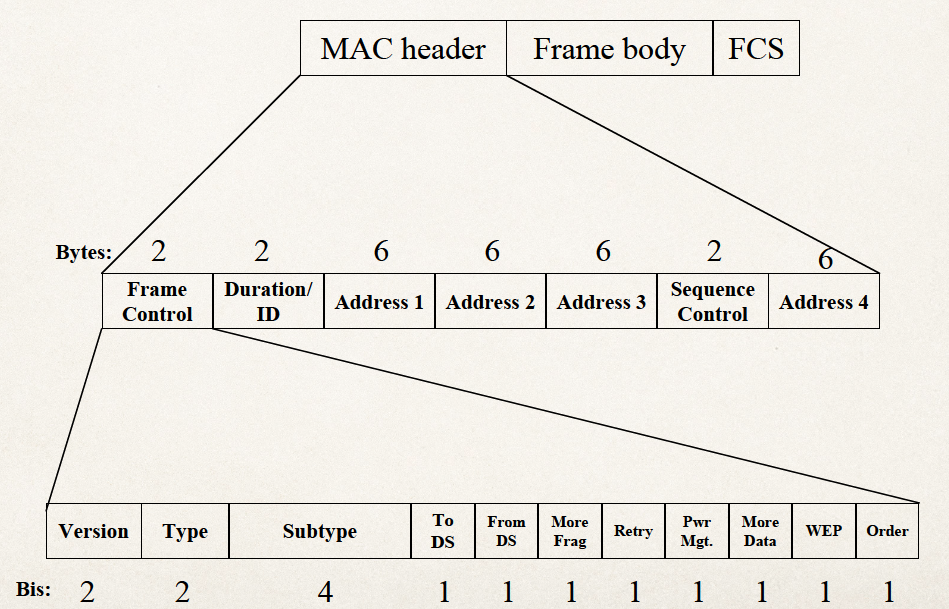
\includegraphics[width=14cm]{images/probe/mac_frame.png}
	\caption{Structure d'une trame MAC}
	\label{fig:macframe}
\end{figure}

On retrouve notamment les adresses MAC de source et de destination dans les champs Address[1|2|3].
Malheureusement, pour qu'un appareil diffuse des trames de \textbf{données}, il faut qu'il soit associé avec un point d'accès. 
Il existe cependant les trames de \textbf{management}. Le champ "Subtype" (cf figure \ref{fig:macframe}) définit justement
la nature de ces frames. 

Voici les trames de management principales:
\begin{itemize}
    \item Beacon
    \item Probe request \& response
    \item Authentification
    \item Association request \& response
    \item Re-association request \& response
    \item Disassociation
    \item De-Authentification
\end{itemize}

Les trames \textbf{Beacon} sont utilisées par les points d'accès pour signaler leur existence. 

Les trames d'\textbf{(De-)Authentification} sont utilisées par une station et un point d'accès afin d'établir leur identité (pas de chiffrement à ce stade).

Les trames d'\textbf{(Dis|Re)Association} sont utilisées pour lier un AP et une station après l'authentification.

Les trames de \textbf{Probing} servent à un client (request) à demander à un AP les informations nécessaires à la connexion (e.g le canal).
L'AP concerné envoie alors une probe response avec les informations. 

Une probe request peut être dirigée (un SSID spécifique est spécifié, on l'appelle alors "directed probe request") ou alors aucun SSID n'est spécifié, dans ce cas
on l'appelle "null probe request"

Pour notre solution de scanning, nous cherchons une trame qui n'a pas d'interaction direct avec un access point préexistant
et qui est envoyée par le client. Parmi les trames de management mentionnées, seules les probe requests respectent ces deux contraintes.

Un autre avantage des probe request est que ces dernières sont envoyées très régulièrement (plusieurs fois par minute)
afin de permettre à l'appareil de trouver rapidement les WiFi disponibles. Elles sont même envoyées en rafale ("burst") afin de couvrir
un maximum de canaux 802.11.

Une capture de probe request dirigée peut être observée sur la capture~\ref{fig:directedprobe} :
\begin{figure}[H]
	\centering
	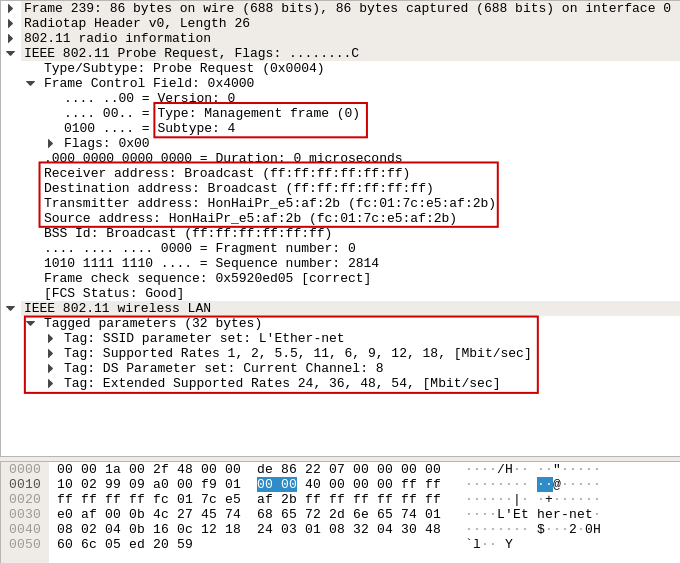
\includegraphics[width=14cm]{images/probe/directed_probe.png}
	\caption{Probe request dirigée}
	\label{fig:directedprobe}
\end{figure}

On y trouve le sous-type de la trame de management qui identifie les Probe requests (4), l'adresse de destination (broadcast)
, l'adresse source (un téléphone Honor 8) et différentes informations dont le \textbf{SSID} recherché : "L'Ether-net"

Les même informations sont disponibles pour une null probe request (figure~\ref{fig:nulldprobe}), mais le SSID est remplacé par un wildcard:
\begin{figure}[H]
	\centering
	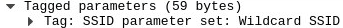
\includegraphics[width=14cm]{images/probe/null_probe_cropped.png}
	\caption{null-probe request}
	\label{fig:nulldprobe}
\end{figure}

Il est intéressant de noter que des informations peuvent parfois être déduites des probes requests dirigées.
La plupart du temps, les requêtes sont dirigées car l'appareil s'est déjà connecté au réseau concerné. 
Si le nom du réseau est connu et assez unique, il devient alors possible de déduire où l'appareil se situait par le passé.
Par exemple, sur la figure \ref{fig:directedprobe}, le SSID est l'ancien nom de mon réseau, je peux donc en déduire qu'il s'agit
d'un de mes appareils, et qu'il n'est pas récent. 

Cette technique est aussi utilisée afin de découvrir des réseaux cachés (il s'agit de réseaux qui ne répondent pas aux null probe requests et qui n'envoient pas de beacons).



\chapter{Implémentation}
\label{ch:implémentation}

\section{La base de données}

\section{L'API WiFace}

\subsection{Choix de la stack}

Du côté serveur, le langage utilisé est le Python (3.7). Pour faciliter le développement d’une API rest, le micro-
framework \textbf{Flask} a été choisi. Au vu de la documentation et de mon expérience personnelle, ce choix est pertinent
dans le cadre de ce projet.

Avantages de Flask :
\begin{itemize}
\item Simple et léger
\item Convient bien au développement d’application de petite ou moyenne envergure
\item Très flexible
\item Prise en main rapide
\item Compatible avec l’ORM sqlalchemy
\end{itemize}

L’ORM qui a été choisi pour fonctionner avec Flask est \textbf{SQLAlchemy}. Il existe en effet un module python flask-
sqlalchemy qui rend l’intégration simple.
Les données sont sérialisées à l’aide de \textbf{marshmallow}.
La gestion de l’authentification se fait à l’aide de token JWT et du module correspondant \textbf{flask-jwt} et \textbf{pyjwt}
La spécification est écrite à l’aide de swagger, qui propose également une documentation automatique.

\section{Le client Raspberry}

\section{Algorithme PP2I}

\chapter{Tests du prototype}
\label{ch:test}

Les tests sont une partie importante de tout projet.
Cependant, pour des raisons éthiques (voir chapitre \ref{ch:etudemoralite}), légales (voir chapitre \ref{ch:etudelegislation}) et logistiques (à cause des mesures de confinement depuis mars 2020)
il a été impossible de tester les divers aspects du prototype en conditions réelles.

\section{Tests de l'algorithme PP2I}
La partie la plus critique à tester est celle concernant l'algorithme PP2I. 
En effet, c'est le point pouvant causer le plus d'erreurs lors du processus.
C'est pourquoi un module de \textbf{simulation} a été développé. 

\subsection{Explication de la simulation}
La simulation est exécutée à la création de la base de donnée.
Selon les paramètres passés au script de création, un certain nombre d'identités vont être générées. 
À chaque identité est associée une adresse MAC connue. 
Une boucle d'événement est exécutée à chaque unité de temps de la simulation (une minute)   
Durant cette boucle, chaque identité à une certaine probabilité d'émettre une probe request contenant son adresse MAC ou 
d'être "pris en photo". Lorsque la simulation est terminée, toutes ces données sont analysées et la correspondance des couples Adresse MAC - Identité est faite. 

Comme nous connaissant la véritable adresse de chaque identité, nous pouvons calculer un taux de réussite correspondant au nombre d'identités ayant reçu la bonne adresse MAC par rapport au nombre d'identités total.

\subsection{Exemple de graphique résultant de la simulation}
Les informations clés de la simulation sont compilées dans un graphique au format de la figure \ref{fig:simulation-result-example} 
\begin{figure}[H]
	\centering
	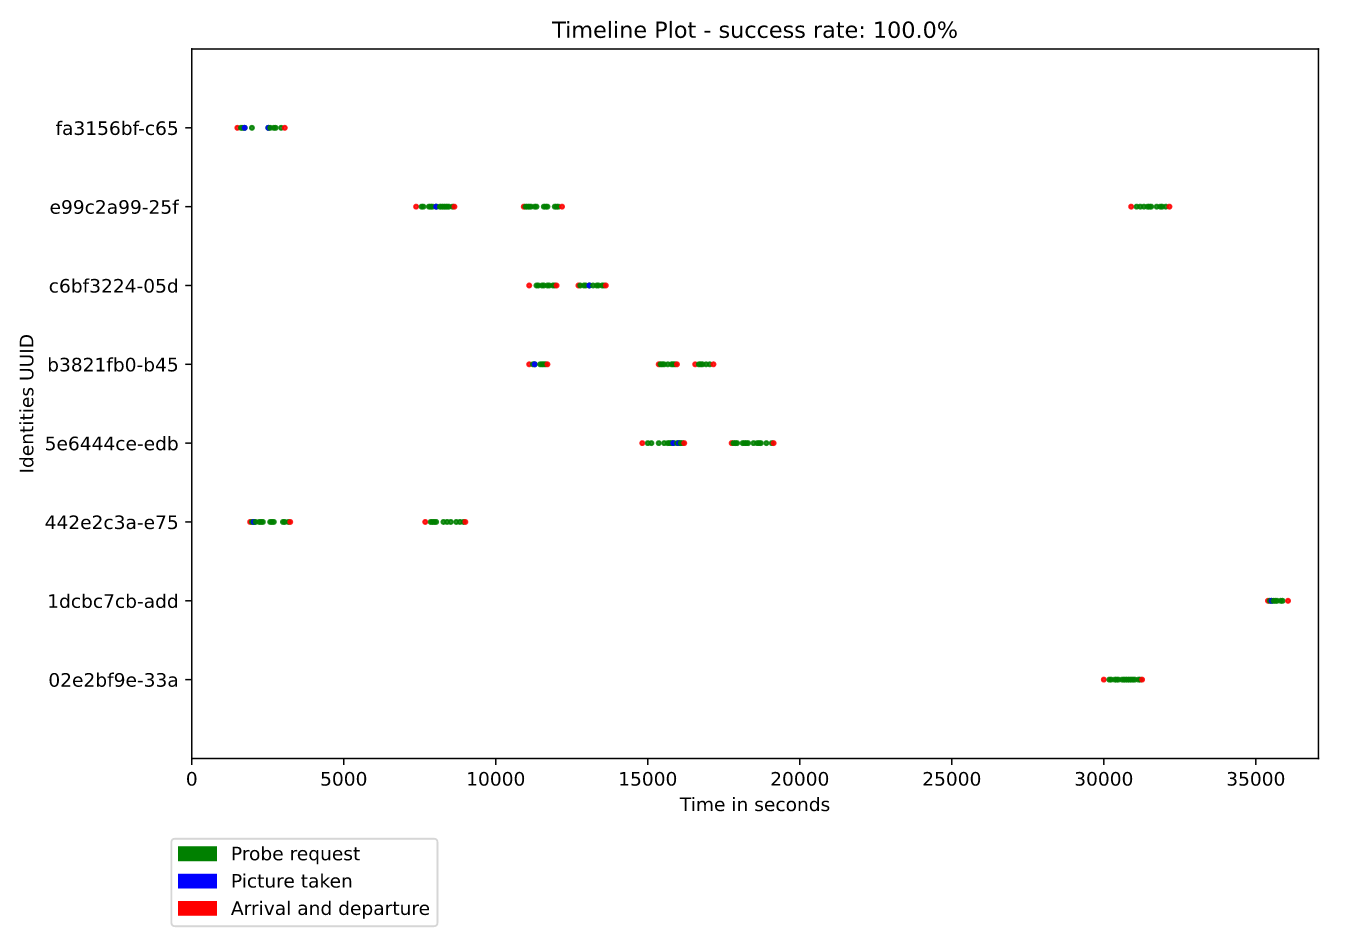
\includegraphics[width=12cm]{images/tests/exemple-graph.png}
	\caption{Exemple de résultat de la simulation}
	\label{fig:simulation-result-example}
\end{figure}

Voici les éléments importants du graphique et leur signification:
\begin{itemize}
    \item Le titre du graphique indique le taux de réussite
    \item L'axe des abcisses indique le déroulement du temps lors de la simulation
    \item L'axe des ordonnées indique un identifiant unique par identité (UUID). Un UUID en rouge indique que l'algorithme PP2I n'a pas assigné la bonne adresse MAC à cette identité 
    \item Chaque point sur la frise chronologique indique un événement dont la couleur indique la nature
\end{itemize}

\subsection{Choix d'implémentation}
Pour simuler au mieux les tests qui auraient pu être effectués en condition réelle, les décisions suivantes ont été prises:

Chaque visite d'une personne est modélisée selon une distribution normale (comme le temps de visite moyen dans un centre commercial par exemple) selon la fonction
\[f(x)=\frac{1}{\sqrt{2\pi \sigma^2}} e^{-\frac{1}{2\sigma^2}(x-\mu)^2}\]

\begin{tikzpicture}
\begin{axis}[every axis plot post/.append style={
  mark=none,domain=0:40,samples=50,smooth},
    % All plots: from -2:2, 50 samples, smooth, no marks
  axis x line*=bottom, % no box around the plot, only x and y axis
  axis y line*=left, % the * suppresses the arrow tips
  enlargelimits=upper,
  legend style={at={(0,-0.15)},anchor=west}] % extend the axes a bit to the right and top
  \addplot {gauss(20,5)};
  
  \addlegendentry{$\sigma$ = 5 et $\mu$ = 20}
\end{axis}
\end{tikzpicture}

Une personne peut faire entre une et quatre visite par simulation.
La distribution discrète de probabilité diminue exponentiellement, puisqu'il est peu probable que quelqu'un décide de revenir:

\tikzset{
  % define the bar graph element
  bar/.pic={
    \fill (-.1,0) rectangle (.1,#1) (0,#1) node[above,scale=1/2]{$#1$};
  }
}
  \begin{tikzpicture}[y=5cm]
    \draw
      % the main axis
      (1,0) edge[-latex] (5,0)
      % draw the distribution and label it
      foreach[count=\i from 1] ~ in {0.64391426, 0.23688282, 0.08714432, 0.0320586}{
        (\i,0) pic[red]{bar=~} node[below]{$\i$}
      };
  \end{tikzpicture}

La probabilité à chaque minute de sniffer une probe request est de 60\%, et de 5\% pour les photos. (Il est bien plus difficile de prendre une photo du visage que de 
capter une paquet à distance.) Il est à noté qu'il s'agit d'une estimation.

\section{Protocole de test}
Deux paramètres vont grandement influencer le résultat et vont guider les tests:
\begin{enumerate}
    \item La durée de la simulation
    \item Le nombre d'identités pouvant se présenter
\end{enumerate}

Six tests vont être effectués, avec un exemple commenté pour chaque catégorie: 
\begin{enumerate}
    \item Fréquentation faible pour une simulation de durée courte
    \item Fréquentation moyenne pour une simulation de durée courte
    \item Fréquentation élevée pour une simulation de durée courte
    \item Fréquentation faible pour une simulation de durée longue
    \item Fréquentation moyenne pour une simulation de durée longue
    \item Fréquentation élevée pour une simulation de durée longue
\end{enumerate}

Chaque test va être exécuté plusieurs fois, et les graphiques résultants seront exportés. 
\section{Tests}
\begin{itemize}
    \item La fréquentation faible est représentée par 10 identités.
    \item La fréquentation moyenne est représentée par 50 identités.
    \item La fréquentation élevée est représentée par 150 identités.
\end{itemize}
\begin{itemize}
    \item Une durée courte est représentée par 5h.
    \item Une durée longue est représentée par 30h.
\end{itemize}


\subsection{Fréquentation faible pour une simulation de durée courte}
Pour ce test, la moyenne est de 83.85\% et la médiane est de 81.25\%.
La durée courte engendre des visites simultanées, ce qui rend impossible l'assignation de certaines adresse, mais
le nombre limité de personne mitige ce phénomème. 

Sur la figure \ref{fig:simulation-short-low} on peut toutefois voir que la première identité a reçu la mauvaise adresse.
C'est sûrement car ses événements sont presque un sous-ensemble de ceux émis par la troisième identité.

On peut également observer qu'il n'y a que 6 identités sur cette expérience. C'est car il y a 4 identités
qui n'ont pas émis de photos, et qui ne sont donc pas considérés par l'algorithme.

\begin{figure}[H]
	\centering
	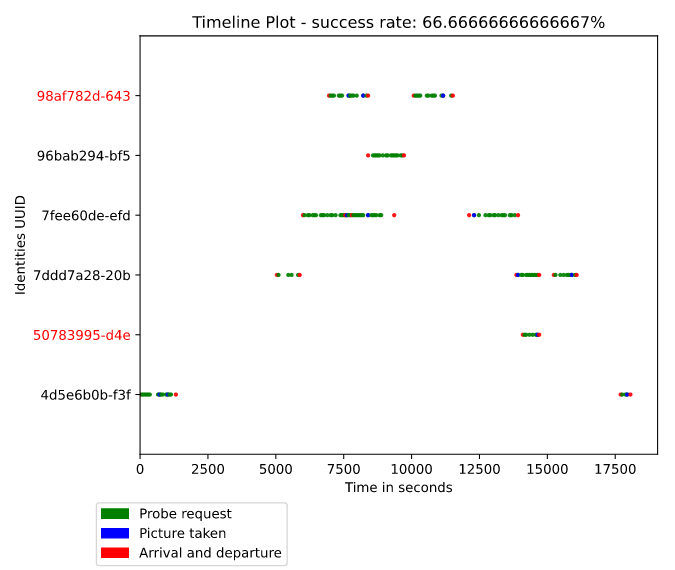
\includegraphics[width=12cm]{images/tests/exemple_courte_faible.png}
	\caption{Exemple de résultat de la simulation à durée courte et fréquentation faible}
	\label{fig:simulation-short-low}
\end{figure}

\subsection{Fréquentation moyenne pour une simulation de durée courte}
Pour ce test, la moyenne est de 61.25\% et la médiane est de 60.52\%.

Les résultats diminuent par rapport au test précédent car le risque de "collisions" augmente.

\subsection{Fréquentation élevée pour une simulation de durée courte}
Pour ce test, la moyenne est de 41.18\% et la médiane est de 41.88\%.

Ce cas de test est le pire de notre matrice. Il devient alors nécessaire d'attendre de nouvelles visites des identités
repérées pour pouvoir être convaincu de résultat de l'algorithme. Heureusement, le but du dispositif WiFace est d'être placé sur le long terme, rendant envisageable la capture des
visites suivantes.

\subsection{Fréquentation faible pour une simulation de durée longue}
Pour ce test, la moyenne est de 96.25\% et la médiane est de 100\%.

Les événements "se diluent" dans une grande période, ce qui rend très fiable l'algorithme. 
Cependant, certains exécutions n'atteigne pas la perfection. On pourrait par exemple considérer le cas d'une 
visite de groupe. Chaque membre va potentiellement émettre des probes requests simultanément, rendant inefficace la détection.
Une telle occurence pourrait être imagée par les deux identités en rouge sur la figure \ref{fig:simulation-long-low}
\clearpage
\newpage
\thispagestyle{empty}
\begin{landscape}
    \centering
\thispagestyle{empty}
\begin{figure}[h]
	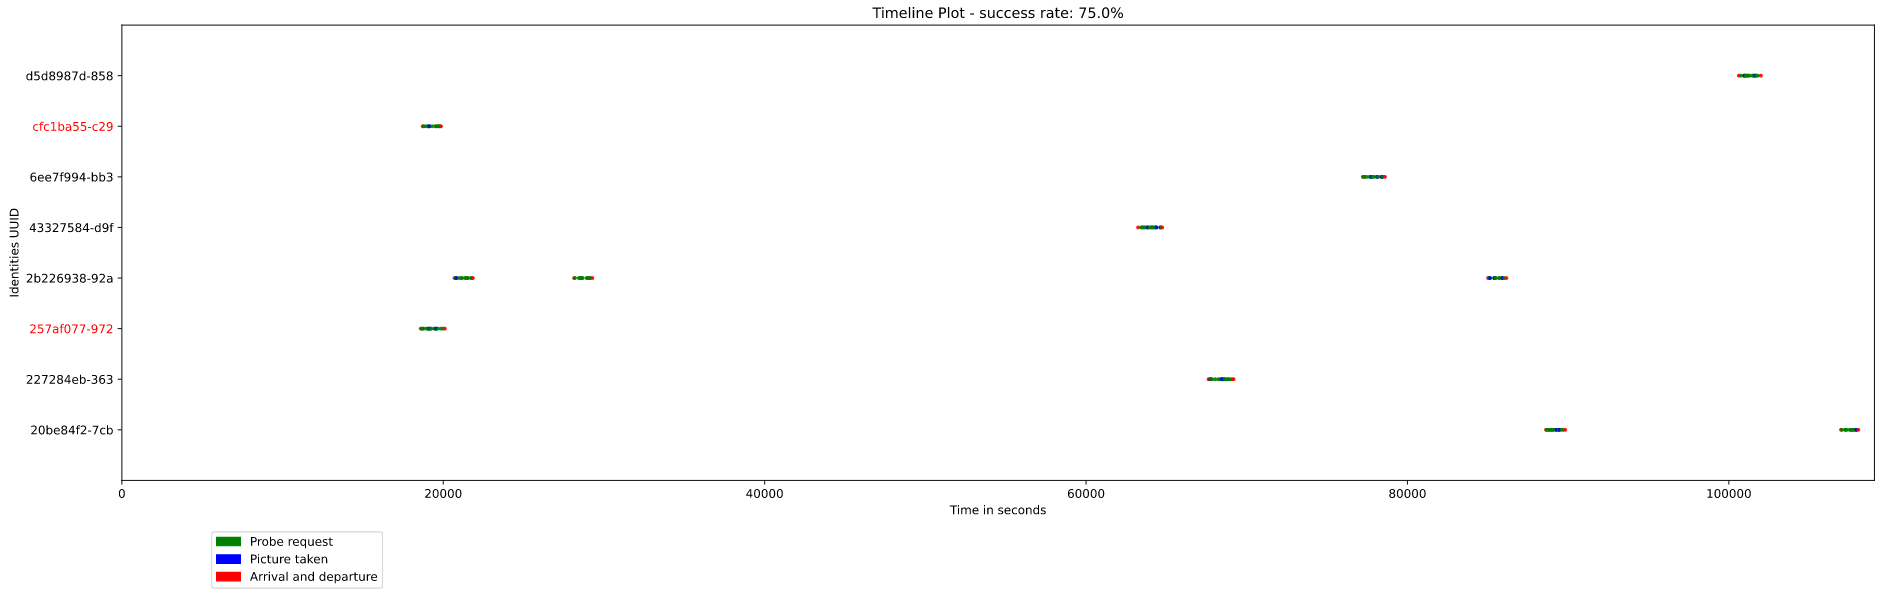
\includegraphics[width=\linewidth]{images/tests/exemple_longue_faible.png}
	\caption{Exemple de résultat de la simulation à durée courte et fréquentation faible}
	\label{fig:simulation-long-low}
\end{figure}
\end{landscape}

\subsection{Fréquentation moyenne pour une simulation de durée longue}
Pour ce test, la moyenne est de 84.43\% et la médiane est de 86.48\%.
Les résultats sont satisfaisants et bien meilleurs qu'en durée courte.

\subsection{Fréquentation élevée pour une simulation de durée longue}
Pour ce test, la moyenne est de 74.58\% et la médiane est de 75\%.

Il s'agit du cas d'utilisation du système le plus probable. 
Posé sur le long terme (bien plus que 30h, mais cette durée a été choisie pour faciliter la simulation), beaucoup de gens fréquenterait l'endroit d'action du dispositif.

\subsection{Synthèse des résultats}

Le tableau \ref{tab:synthese_pp2i} résume les résultats obtenus lors des tests.

\begin{table}[H]
    \begin{tabular}{lllll}
                          & \multicolumn{2}{c}{Durée courte} & \multicolumn{2}{c}{Durée longue} \\
                          & Moyenne         & Médiane        & Moyenne        & Médiane         \\
    Fréquentation faible  & 83.85\%         & 81.25\%        & 96.25\%        & 100.00\%        \\
    Fréquentation moyenne & 61.25\%         & 60.52\%        & 84.43\%        & 86.48\%         \\
    Fréquentation forte   & 41.18\%         & 41.88\%        & 74.58\%        & 75.00\%        
    \end{tabular}
\caption{Synthèse des résultats des tests PP2I}
\label{tab:synthese_pp2i}
\end{table}

Pour conclure, nous pouvons affirmer que les résultats sont satisfaisants et démontre une valeur ajoutée de l'algorithme PP2I. 
Il existe toutefois divers problèmes qui n'ont pas pu être résolu et qui baisse les performances. Parmi ces problèmes, il y a notamment:
\begin{itemize}
    \item Les visites de groupes qui rendent indiscernables les membres individuellement (sauf si une nouvelle visite séparée du groupe se produit)
    \item Lorsque la période d'activité est trop saturée (peu de temps ou grande fréquentation)
    \item Il est difficile de prendre des photographies (ce qui a été simulé avec un petit pourcentage), ce qui amène parfois à des nuages de points représentant des probe requests, sans image, faussant ainsi le calcul du score.
    \item Les adresses MAC aléatoires ne sont implémentées dans la simulation mais aurait comme conséquence l'ajout de bruit dans la détection 
\end{itemize}







\chapter{Guides d'installation}
\label{ch:guide_installation}

Ce chapitre traitera de l'installation de tous les composants de l'architecture comprenant notamment: 
\begin{itemize}
    \item Le serveur Flask
    \item La base de données SQLite partiellement peuplée
    \item Le(s) client(s) Raspberry Pi avec leurs modules (PiCaméra et antenne 802.11)
\end{itemize}
Toutes ces étapes seront séparées en deux parties: un guide pour le client, et un guide pour le serveur 
\section{Installation du serveur WiFace}
Pour rappel, le serveur WiFace ou "WiFace API" (cf \ref{fig:diag_archi}) endosse les responsabilités
suivantes: 
\begin{itemize}
    \item Récolte, persiste, et traite les données envoyées par les clients (Raspberry ou utilisateur front-end)
    \item Fourni de l'authentification
    \item Offre une API
    \item Offre une interface web pour les opérateurs humains
    \item Interagit avec les systèmes externes nécessaire au traitement des données (e.g AWS Rekognition)
\end{itemize}

\subsection{Prérequis software}
\begin{itemize}
    \item Docker : Le serveur est dockerisé afin de faciliter l'installation
    \item git: Les fichiers nécessaires se trouve sur github
\end{itemize}

\subsection{Marche à suivre}
La marche à suivre pour exécuter le serveur est la suivante:
\begin{enumerate}
    \item Clôner le repository \textbf{TB WiFace}
    \begin{listingsbox}{console}{Clônage du dépôt sur github}
git clone https://github.com/Obyka/TB_WiFace.git
    \end{listingsbox}
    \item{Se déplacer dans le sous-dossier API}
    \item{Configurer le script de démarrage start.sh}
\end{enumerate}
    Il existe deux modes pour la création de la base de donnée. Le premier
    consiste à inclure quatres identités inscrites dans le script build\_database.py.
    Le deuxième consiste à lancer une simulation pour l'algorithme PP2I et d'y inscrire les résultats.
    Les paramètres de la simulation peuvent être ajusté dans le script start.sh
    
\begin{listingsbox}{console}{Exemple de configuration de start.sh}
#!/bin/bash
simulation=0
nb_person=10
duration=1000

if [[ $simulation -eq 1 ]];
then
    python build_database.py --nb_person $nb_person \
    --duration $duration --simulation && python3 server.py
else
    python3 build_database.py && python3 server.py
fi    
\end{listingsbox}
    
\begin{enumerate}[resume]
    \item Modifier le fichier API/config.py. Plusieurs constantes relatives à la sécurité doivent être modifiées (credentials Amazon, JWT et CSRF secrets)
    \item Modifier l'utilisateur par défaut dans le fichier API/build\_database.py et s'assurer qu'il soit bien admin.
\end{enumerate}

\begin{enumerate}[resume]
    \item Construire l'image docker correspondante et la démarrer.
\end{enumerate}

Le build peut prendre quelques minutes afin d'obtenir les dépendances python.
Ici, le port 5555 sera exposé.
\begin{listingsbox}{console}{Création et démarrage de l'image docker}
docker build -t wiface-api .
docker run -p 5555:5000 wiface-api
\end{listingsbox}

Le serveur est maintenant disponible aus adresses api/ et web/.

\section{Installation d'un client Raspberry Pi}
Cette section détaille l'installation, la configuration et l'utilisation d'un client Raspberry Pi.

\subsection{Prérequis}

\subsubsection{Prérequis hardware}
\begin{itemize}
    \item Une Raspberry Pi 4 Model B avec 4GB de RAM
    \item Un module Pi Camera v2
    \item Une antenne 802.11 compatible avec le mode Monitor
\end{itemize}

\subsubsection{Prérequis software}
\begin{itemize}
    \item Raspbian 10 (Buster)
    \item Python 3.7.3
\end{itemize}

\subsection{Création du compte local}
Afin de réduire la surface d'attaque, un compte va être créé pour ne pas utiliser
le profil par défaut (pi).
La commande sudo sera aussi configurée pour demander systèmatiquement un mot de passe.
Ce compte sera ensuite ajouté au groupe sudo, ce qui est nécessaire pour utiliser Scapy.
Pour des raisons pratiques, le mot de passe utilisé sera inscrit dans ce rapport. En cas d'utilisation de WiFace, merci de changer ce dernier.

Le compte par défaut ne devrait pas être supprimé, pour des raisons
de dépendances. Son mot de passe doit toutefois être modifié.

\begin{listingsbox}{console}{Création d'un compte local}
# Changer le mot de passe de l'utilisateur pi
passwd

sudo adduser wiface-user
New password: Mu7%0&J#0!X^&t6OHHQ@z&
sudo usermod -a -G adm,dialout,cdrom,sudo,audio\
,video,plugdev,games,users,input,netdev,gpio,i2c,spi wiface-user

# Changer les lignes correspondantes à Pi et wiface-user par 
# pi ALL=(ALL) PASSWD: ALL
sudo visudo /etc/sudoers.d/010_pi-nopasswd
\end{listingsbox}

Pour faciliter la gestion du client, une paire de clé ssh va être créée pour permettre la connexion distante.
Pour cela, il faut activer le serveur ssh sur le client et copier la clé publique dessus.

\begin{listingsbox}{console}{Ajout d'une clé SSH}
    # Activer SSH sous "Interfacing options"
    sudo raspi-config

    # Sur le PC qui va se connecter au client
    ssh-keygen
    ssh-copy-id wiface-user@<IP-ADDRESS>
    ssh wiface-user@<IP-ADDRESS>

    # Il faut désactiver la connexion par mot de passe pour
    # profiter de la sécurité offerte par les clés ssh.
    sudo nano /etc/ssh/sshd_config
    ChallengeResponseAuthentication no
    PasswordAuthentication no
    UsePAM no

    # Relancer le service
    sudo service ssh reload
\end{listingsbox}

\subsection{Installation des dépendances}
Maintenant que la configuration est faite, il faut installer les dépendances
nécessaires à l'exécution du client. 

\begin{listingsbox}{console}{Installation des dépendances du client}
    sudo pip3 install --pre scapy[basic]
    sudo pip3 install requests
\end{listingsbox}


\subsection{Installation de l'antenne 802.11}
Pour faire fonctionner l'antenne en mode "Monitor", nous allons utiliser Aircrack-ng.\footnote{Aircrack-ng est une suite de logiciel permettant des opérations sur les périphériques, protocoles, et réseau WiFi.}
\begin{listingsbox}{console}{Installation de aircrack-ng}
sudo apt-get update
sudo apt-get upgrade
sudo apt-get install aircrack-ng

# Si le programme a été installé correctement, la commande
# devrait retourner les différentes interfaces réseaux.
sudo airmon-ng
\end{listingsbox}

Une fois l'antenne connectée, la dernière commande devrait retourner une ligne supplémentaire. 
Cela veut dire que le périphérique a bien été détecté, nous pouvons donc le passer en mode Monitor.

\begin{listingsbox}{console}{Passage de l'interface en mode Monitor}
sudo airmon-ng start <Interface-Name>
\end{listingsbox}

L'interface est maintenant prête pour le scan.

\subsection{Installation du module PiCamera}
Après avoir connecté le module caméra, quelques installations et configurations sont nécessaires.

\begin{listingsbox}{console}{Installation de la picamera}
    # Installation du module python
    sudo apt-get install python-picamera python3-picamera

    # Activer Camera sous "Interfacing options" et accepter le reboot
    sudo raspi-config 
\end{listingsbox}

Afin de reconnaître les visages, OpenCV est utilisé sur le client.
Voici son installation\cite{OPENCVINSTA}. Nous compilons les sources car cela permet d'avoir
toutes les fonctionnalités. 
\begin{listingsbox}{console}{Installation d'OpenCV}
# Nettoyage de paquets inutiles afin de gagner de l'espace de stockage

$ sudo apt-get purge wolfram-engine
$ sudo apt-get purge libreoffice*
$ sudo apt-get clean
$ sudo apt-get autoremove

$ sudo apt-get update && sudo apt-get upgrade

$ sudo apt-get install build-essential cmake pkg-config

$ sudo apt-get install libjpeg-dev libtiff5-dev \
    libjasper-dev libpng-dev libqt4-test
$ sudo apt-get install libavcodec-dev libavformat-dev \ 
    libswscale-dev libv4l-dev
$ sudo apt-get install libxvidcore-dev libx264-dev
$ sudo apt-get install libfontconfig1-dev libcairo2-dev
$ sudo apt-get install libgdk-pixbuf2.0-dev libpango1.0-dev
$ sudo apt-get install libgtk2.0-dev libgtk-3-dev
$ sudo apt-get install libatlas-base-dev gfortran
$ sudo apt-get install libhdf5-dev libhdf5-serial-dev libhdf5-103
$ sudo apt-get install libqtgui4 libqtwebkit4 libqt4-test python3-pyqt5
$ sudo apt-get install python3-dev

$ cd ~
$ wget -O opencv.zip https://github.com/opencv/opencv/archive/4.1.1.zip
$ wget -O opencv_contrib.zip \ 
    https://github.com/opencv/opencv_contrib/archive/4.1.1.zip
$ unzip opencv.zip
$ unzip opencv_contrib.zip
$ mv opencv-4.1.1 opencv
$ mv opencv_contrib-4.1.1 opencv_contrib

# Augmenter le SWAP pour accélerer l'installation. 
# CONF_SWAPSIZE=2048
$ sudo nano /etc/dphys-swapfile
# Redémarrage du service
$ sudo /etc/init.d/dphys-swapfile stop
$ sudo /etc/init.d/dphys-swapfile start

$ pip install numpy

$ cd ~/opencv
$ mkdir build
$ cd build
$ cmake -D CMAKE_BUILD_TYPE=RELEASE \
    -D CMAKE_INSTALL_PREFIX=/usr/local \
    -D OPENCV_EXTRA_MODULES_PATH=~/opencv_contrib/modules \
    -D ENABLE_NEON=ON \
    -D ENABLE_VFPV3=ON \
    -D BUILD_TESTS=OFF \
    -D INSTALL_PYTHON_EXAMPLES=OFF \
    -D OPENCV_ENABLE_NONFREE=ON \
    -D CMAKE_SHARED_LINKER_FLAGS=-latomic \
    -D BUILD_EXAMPLES=OFF ..

$ make -j4
$ sudo make install
$ sudo ldconfig

# Ne pas oublier de reset le SWAP.
\end{listingsbox}
    




\chapter{Conclusion}
\label{ch:conclusion}

\section{Difficultés rencontrées}
Ce travail étant le premier de cette ampleur que j'effectue, j'ai été
confronté à quelques difficultés que je souhaite énumérer ici.

\subsection{Problèmes liés au Covid-19}
Depuis mars 2020, la pandémie SARS-CoV-2 a complétement changé la façon
de travailler et ce jusqu'à la fin de mon travail de Bachelor en juillet 2020.

Ces changements ont apportés quelques complications:

\subsubsection{Complication des tests}
À cause de l'interdiction de se rassembler, et également pour les raisons légales et morales (cf \ref{ch:etudelegislation} et \ref{ch:etudemoralite}),
il ne m'a pas été possible de tester mon produit en situation réelle, menant à avoir quelques réserves quant à son efficacité effective.

Le module de simulation développé pour pallier ce problème a toutefois permis de tester d'autres aspects qui ne l'auraient pas été en condition réelle, comme un très grand nombre
de personnes, ou une simulation de plusieurs dizaines d'heures. 

\subsubsection{Cadre de travail et motivation}
Étant confiné pendant la majeure partie de mon travail, il a parfois été compliqué
d'entretenir une motivation sur le long terme à cause de l'isolement et du climat parfois anxiogène.

\subsection{Le matériel}

\subsubsection{PiCaméra défectueuse}
Après quelques semaines d'utilisation, un des modules PiCamera a arrêté de fonctionner.
Il semblerait que cela soit un disfonctionnement matériel. Cet incident m'a fait perdre du temps à cause du dépannage et de la nouvelle commande.

\section{Améliorations futures}
Dans le futur, ces quelques idées pourraient être implémentées pour étendre les capacités du prototype ou l'améliorer.
\begin{itemize}
    \item Ajouter un serveur WSGI devant l'API et le front-end afin de rendre le produit plus "production-friendly"
    \item Améliorer l'algorithme PP2I pour en diminuer la complexité algorithmique
    \item Analyser les implémentations actuelles de la randomisation d'adresses MAC afin de trouver de nouvelles contre-mesures
    \item Ajouter un module permettant l'attaque active (e.g~\cite{WIFIKARMA}) sur les clients raspberry (e.g une autre interface pouvant créer des evil twins)
    \item Développer un mode "privacy-friendly" qui ne permettraient aux opérateurs du système de n'effectuer que des statistiques de masse sans connaître d'informations individuelles
\end{itemize}

\section{Retour personnel}
Ces quelques mois de travail ont été très enrichissants.
Tout d'abord, il s'agit du travail le plus personnel qui m'a été donné de faire.
Habitué à des travaux de groupe, j'ai pu goûter à une nouvelle forme d'autonomie, ce qui m'a permis de fournir
un projet dont je suis fier et dont je maîtrise chaque partie. 

Je suis satisfait des résultats obtenus lors des diverses étapes du projet, notamment ceux concernant l'algorithme PP2I que j'ai conçu.
J'ai toutefois été un peu déçu de ne pas avoir pu m'attaquer à la randomisation des adresses MAC, par manque de temps et de ressources.

Je suis également surpris de la facilité avec laquelle il a été possible d'inclure des services de reconnaissance faciale au projet. Je n'imaginais pas
que l'état de l'art permettait cela avec mes connaissances actuelles.

\section{Remerciements}

Je souhaite évidemment remercier toutes les personnes ayant contribué à la réussite de mes
études, et de ce travail de Bachelor en particulier.

En tout premier lieu, je tiens à remercier mon responsable de travail: Monsieur Abraham Rubinstein.
De par ses précieux conseils, son suivi régulier ainsi que son optimisme lors d'une période compliquée pour tous, il m'a permis
d'affirmer au mieux mes compétences, et ainsi de rendre un travail dont je suis fier.

Je souhaite également adresser ma gratitude à tous les professeurs qui ont investi de leur temps et leurs efforts pour
guider mes camarades et moi vers l'obtention de notre diplôme. J'ai énormément appris pendant ce Bachelor grâce à leur travail exceptionnel.

Pour leur patience, et tout ce qu'ils m'ont donné, je renouvelle dans ce document, le respect, l'amour et la gratitude que j'éprouve pour mes parents, Corinne et Philippe Polier.
Toujours encourageants, c'est leur soutien indéfectible qui fait de moi l'étudiant et la personne que je suis aujourd'hui.

Pour conclure, je remercie et adresse mes voeux à mes camarades. 
Travailler avec eux a été une source inépuisable de motivation et je leur souhaite à tous la réussite professionelle.
Certains d'entre eux ont activement collaborés à mon travail: Notamment Julien Quartier, qui m'a offert un peu de son temps ainsi que ses connaissances
en m'imprimant le support des modules PiCamera.





% +---------------------------------------------------------------+
\cleardoublepage
\addcontentsline{toc}{chapter}{Bibliographie}
\bibliographystyle{plain}
\bibliography{chapters/biblio}
\nocite{*} %ajoute tout ce qu'il y a dans le bibtex

\listoffigures
\listoftables

% Annexes
% +---------------------------------------------------------------+
\appendix

\end{document}
